\documentclass[11pt,a4paper]{article}
\usepackage[T1]{fontenc}
\usepackage[utf8]{inputenc}
\usepackage[brazil]{babel}
\usepackage{lmodern}
\usepackage{microtype}
\usepackage[a4paper,left=25mm,right=25mm,top=26mm,bottom=25mm,headheight=16pt]{geometry}
\usepackage{amsmath,amssymb}
\usepackage[table]{xcolor}
\usepackage{graphicx,float,caption,booktabs,tabularx,array}
\usepackage{enumitem,setspace,fancyhdr,titlesec,listings,pdfpages}
\usepackage[unicode,colorlinks=true,linkcolor=tcdnavy,urlcolor=tcdteal,bookmarksnumbered=true]{hyperref}
\definecolor{tcdnavy}{gray}{0}
\definecolor{tcdteal}{gray}{0}
\definecolor{tcdgray}{gray}{0}
\definecolor{tcdlight}{gray}{0.96}
\definecolor{tcdtablehead}{gray}{0.86}
\pdfstringdefDisableCommands{\def\times{×}}
\hypersetup{pdftitle={Transmissão confiável de textos e imagens via RF 433 MHz},pdfauthor={Enzo Aurélio de Alvarenga Gomes; Enzo Christyan Mubarak Oliveira Arruda; Felipe Enzo Fukase}}
\setlength{\parindent}{1.25cm}
\setlength{\parskip}{2.5pt}
\setstretch{1.10}
\setlength{\emergencystretch}{2em}
\setcounter{tocdepth}{2}
\setcounter{secnumdepth}{2}
\setlist[enumerate]{leftmargin=*,topsep=4pt,itemsep=2pt,parsep=0pt}
\titleformat{\section}{\sffamily\Large\bfseries\color{tcdnavy}}{\thesection}{0.65em}{}[\vspace{2pt}\color{tcdteal}\titlerule]
\titleformat{\subsection}{\sffamily\large\bfseries\color{tcdnavy}}{\thesubsection}{0.6em}{}
\titleformat{\subsubsection}{\sffamily\normalsize\bfseries\color{tcdnavy}}{}{0pt}{}
\titlespacing*{\section}{0pt}{8pt}{13pt}
\titlespacing*{\subsection}{0pt}{12pt}{6pt}
\titlespacing*{\subsubsection}{0pt}{8pt}{4pt}
\captionsetup{font={small,sf},labelfont={bf,color=tcdnavy},textfont={color=tcdgray},justification=centering,skip=5pt}
\captionsetup[table]{position=top}
\setlength{\tabcolsep}{5pt}
\renewcommand{\arraystretch}{1.18}
\pagestyle{fancy}
\fancyhf{}
\fancyhead[L]{\small\sffamily\color{tcdgray} IFMT\enspace\textperiodcentered\enspace TCD\enspace\textperiodcentered\enspace RF 433 MHz}
\fancyhead[R]{\small\sffamily\color{tcdgray} Relatório técnico}
\fancyfoot[L]{\footnotesize\sffamily\color{tcdgray} Firmware V7 | Resultados de 24/11/2026}
\fancyfoot[R]{\small\sffamily\thepage}
\renewcommand{\headrulewidth}{0.4pt}
\renewcommand{\footrulewidth}{0.4pt}
\lstset{basicstyle=\ttfamily\small,backgroundcolor=\color{tcdlight},frame=single,rulecolor=\color{black!45},breaklines=true,columns=fullflexible,keepspaces=true,showstringspaces=false,aboveskip=8pt,belowskip=8pt,xleftmargin=4pt,xrightmargin=4pt}
\lstset{literate={á}{{\'{a}}}1 {à}{{\`{a}}}1 {ã}{{\~{a}}}1 {â}{{\^{a}}}1 {é}{{\'{e}}}1 {ê}{{\^{e}}}1 {í}{{\'{i}}}1 {ó}{{\'{o}}}1 {ô}{{\^{o}}}1 {õ}{{\~{o}}}1 {ú}{{\'{u}}}1 {ç}{{\c{c}}}1}
\newcommand{\instituicao}{Instituto Federal de Mato Grosso}
\newcommand{\campus}{Campus Cuiabá -- Octayde Jorge da Silva}
\newcommand{\disciplina}{Transmissão e Comunicação de Dados}
\newcommand{\autores}{Enzo Aurélio de Alvarenga Gomes\\[3pt] Enzo Christyan Mubarak Oliveira Arruda\\[3pt] Felipe Enzo Fukase}
\newcommand{\docente}{Ruy Barbosa}
\begin{document}
\renewcommand{\lstlistingname}{Código}
\hypersetup{pageanchor=false}
\begin{titlepage}
\centering\sffamily
{\large\bfseries\MakeUppercase{\instituicao}\par}
\vspace{3pt}{\large\campus\par}
\vspace{1.8cm}{\large\disciplina\par}
\vfill
{\color{tcdteal}\rule{0.85\linewidth}{1pt}\par}\vspace{0.5cm}
{\huge\bfseries\color{tcdnavy} Transmissão confiável de textos e imagens via rádio de 433 MHz entre dois ESP32\par}
\vspace{0.5cm}{\large CRC-8 \textperiodcentered\ Codificação 4B6B \textperiodcentered\ Stop-and-Wait ARQ\par}
\vspace{0.5cm}{\color{tcdteal}\rule{0.85\linewidth}{1pt}\par}
\vspace{0.7cm}{\large Relatório técnico do projeto final\par}
\vfill
{\large\autores\par}\vspace{0.4cm}{\large Docente: \docente\par}
\vfill
{\large Cuiabá -- MT\par 2026\par}
\end{titlepage}
\hypersetup{pageanchor=true}

\clearpage\section*{Resumo}\addcontentsline{toc}{section}{Resumo}
Este relatório descreve o desenvolvimento, a montagem e a validação de um enlace de comunicação bidirecional entre dois microcontroladores ESP32, por meio de módulos transmissores e receptores de rádio de 433 MHz. Os computadores comunicam-se localmente com os ESP32 via USB, enquanto as placas trocam dados exclusivamente pelo enlace RF. O protocolo implementado em Arduino/C++ utiliza quadros DATA, ACK e END, codificação 4B6B, verificação de integridade CRC-8 e recuperação de falhas por Stop-and-Wait ARQ, com controle de sequência alternada. Scripts Python convertem imagens em bitmaps monocromáticos, realizam a transferência serial e reconstroem os arquivos no destino. O circuito B contém um display OLED SSD1306 para visualização de textos e imagens.

A validação seguiu o protocolo V7 de 23/11/2026, com resultados consolidados em 24/11/2026. Os quatorze ensaios foram executados segundo a equipe; os registros T01–T09 documentam o funcionamento textual, a detecção de corrupção e a recuperação de confirmações. O T06 possui comprovação parcial, pois não há evidência suficiente das duas mensagens previstas. No T10, dez mensagens foram recebidas a 1,12 m; no T11, lotes de dez mensagens foram concluídos com e sem obstáculo. T12, T13 e T14 demonstraram reconstrução de imagens de 256, 1.024 e 256 bytes, respectivamente, com concordância de CRC32 e SHA-256 dos pixels. No T13, a distância foi reduzida durante o envio; no T14, uma tentativa foi interrompida antes da sessão bem-sucedida.

Os resultados demonstram a aplicação prática de enquadramento, detecção de erros, controle de fluxo, retransmissão e comunicação sem fio nos casos observados. O número de reenvios, os descartes 4B6B e a duração das transferências evidenciam limitações de eficiência e estabilidade, não permitindo afirmar imunidade a ruído nem aprovação formal irrestrita de todos os critérios. São apresentados os procedimentos de reprodução, fotografias da montagem, esquemáticos funcionais, contadores, hashes e registros experimentais.

\textbf{Palavras-chave:} ESP32; RF 433 MHz; CRC-8; 4B6B; Stop-and-Wait ARQ; transmissão de imagens.

\subsubsection*{Base documental}
Este texto integra o relatório técnico anterior, o protocolo oficial V7, a documentação do repositório e o relatório de ensaios consolidado de 24/11/2026. Os dados do último documento prevalecem sobre os estados experimentais anteriores. NR significa não registrado. As fotografias e capturas foram recuperadas dos documentos fornecidos pela equipe.

{\small Repositório: \href{https://github.com/enzogomes2006/tcd-rf433-esp32}{github.com/enzogomes2006/tcd-rf433-esp32}\par}
\clearpage
\begingroup\small\setstretch{1.0}\setlength{\parskip}{0pt}\tableofcontents\endgroup
\clearpage
\begingroup\footnotesize\setstretch{1.0}\setlength{\parskip}{0pt}\listoffigures\endgroup
\clearpage
\begingroup\small\setstretch{1.0}\setlength{\parskip}{0pt}\listoftables\endgroup

\clearpage\section{Introdução e objetivos}
A comunicação de dados por rádio está sujeita a atenuação, alterações de bits, perdas de quadros, interferência e atrasos. Em enlaces de baixo custo, a presença de um transmissor e um receptor não garante, por si só, que o conteúdo entregue seja igual ao conteúdo enviado. O projeto da disciplina propõe implementar os mecanismos de uma comunicação confiável entre dois computadores, utilizando dois ESP32 e módulos RF de 433 MHz, sem biblioteca pronta de protocolo RF como RadioHead.

\setcounter{subsection}{0}\subsection{Objetivo geral}
Implementar e demonstrar um sistema de comunicação bidirecional capaz de transmitir textos e imagens, identificar erros, recuperar quadros sem confirmação e evitar a duplicação de dados no receptor.

\setcounter{subsection}{1}\subsection{Objetivos específicos}
\begin{enumerate}
\item Construir dois nós de comunicação, cada um com ESP32, transmissor e receptor de 433 MHz.
\item Implementar enquadramento de dados, FCS por CRC-8, codificação 4B6B e controle de sequência.
\item Aplicar Stop-and-Wait ARQ para transmitir e confirmar cada quadro e retransmitir quando necessário.
\item Integrar o display OLED no circuito B e scripts Python para conversão, envio e reconstrução de imagens.
\item Validar texto, fragmentação, erros simulados, perda de ACK, alcance, obstáculos e transmissão de imagens em ambos os sentidos.
\end{enumerate}
\setcounter{subsection}{2}\subsection{Requisitos e escopo}
O enunciado requer comunicação exclusivamente por rádio entre as placas, distância superior a um metro, entrega íntegra, resistência a perturbações, código publicado, cálculo do FCS e evidências da demonstração. O display empregado é OLED SSD1306, em substituição ao LCD mencionado no enunciado; a aceitação pelo docente precisa ser confirmada. A análise diferencia corrupção simulada de perturbação física e não atribui medições a situações sem registro.


\section{Arquitetura do sistema}
\begin{figure}[H]\centering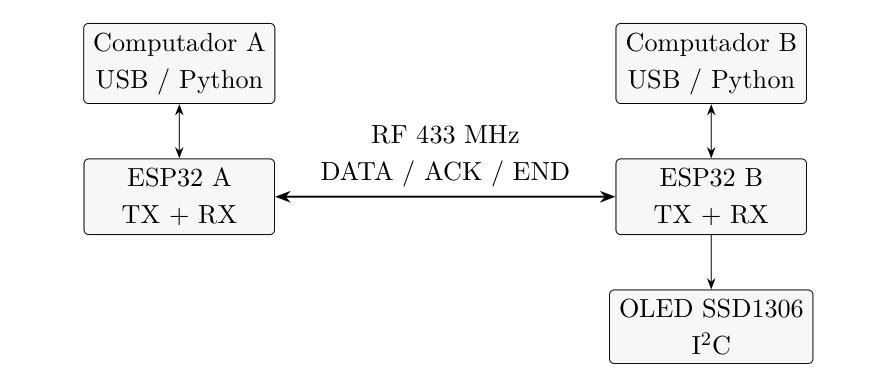
\includegraphics[width=\linewidth,height=210pt,keepaspectratio]{figuras/arquitetura.png}\caption{Arquitetura funcional do enlace bidirecional. Fonte: relatório técnico anterior.}\label{fig:arquitetura}\end{figure}
O computador A envia comandos e bytes por USB ao ESP32 A. O microcontrolador organiza os dados, calcula o FCS, codifica e aciona o transmissor RF. O receptor RF do circuito B entrega os sinais ao ESP32 B, que decodifica, verifica a integridade e confirma os quadros válidos pelo rádio. O computador B recebe o conteúdo reconstruído por USB; o OLED apresenta a informação localmente.

Na direção B \ensuremath{\to} A, os mesmos papéis são invertidos. Cada circuito possui alimentação e referência de terra locais. Não existe conexão física de dados entre A e B. O enlace é utilizado em semiduplex: a aplicação inicia uma sessão de envio por vez para reduzir colisões.

\begin{table}[H]\centering\small\caption{Camada / Função}\label{tab:1}
\rowcolors{2}{tcdlight}{white}\begin{tabularx}{\linewidth}{>{\hsize=0.5567\hsize\linewidth=\hsize\raggedright\arraybackslash}X>{\hsize=1.4433\hsize\linewidth=\hsize\raggedright\arraybackslash}X}
\rowcolor{tcdtablehead} \textcolor{black}{\textbf{Camada}} & \textcolor{black}{\textbf{Função}} \\
Computador /\allowbreak  Python & Interface com usuário, conversão de imagem, USB, reconstrução e hashes. \\
ESP32 /\allowbreak  firmware V7 & Enquadramento, CRC-8, codificação 4B6B, ARQ e controle de sequência. \\
RF TX/\allowbreak RX & Transporte de sinais por rádio de 433 MHz. \\
OLED I\textsuperscript{2}C (somente B) & Apresentação local de texto e imagem monocromática. \\
\bottomrule\end{tabularx}\end{table}

\clearpage\section{Materiais e montagem}
\begin{table}[H]\centering\small\caption{Componentes empregados no projeto}\label{tab:2}
\rowcolors{2}{tcdlight}{white}\begin{tabularx}{\linewidth}{>{\hsize=0.2969\hsize\linewidth=\hsize\raggedright\arraybackslash}X>{\hsize=1.2062\hsize\linewidth=\hsize\raggedright\arraybackslash}X>{\hsize=1.4969\hsize\linewidth=\hsize\raggedright\arraybackslash}X}
\rowcolor{tcdnavy} \textcolor{white}{\textbf{Qtd.}} & \textcolor{white}{\textbf{Componente}} & \textcolor{white}{\textbf{Função}} \\
2 & ESP32 Dev Module & Processamento e interfaces seriais. \\
2 & Transmissor FS1000A, 433 MHz & Envio de dados e confirmações. \\
2 & Receptor RF 433 MHz & Recepção; modelo exato não confirmado. \\
1 & OLED SSD1306 128\ensuremath{\times}64 I\textsuperscript{2}C & Exibição no circuito B. \\
2 & Protoboards & Montagem dos circuitos. \\
2 & Computadores e cabos USB & Alimentação local, programação e comunicação. \\
4 & Condutores de cabo Ethernet & Antenas artesanais TX e RX. \\
Diversos & Jumpers, ferro de solda, solda & Ligações elétricas e fixação das antenas. \\
\bottomrule\end{tabularx}\end{table}
\begin{figure}[H]\centering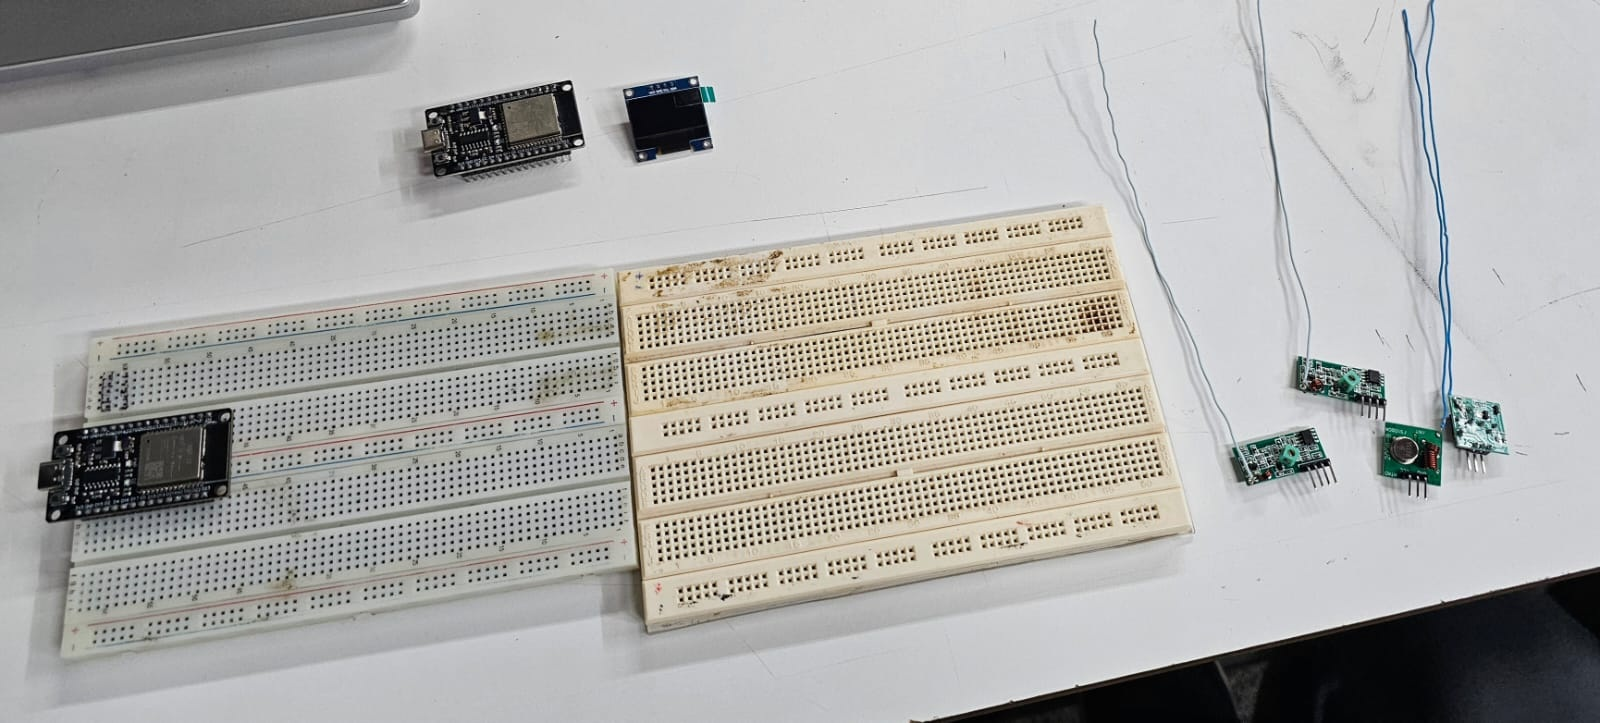
\includegraphics[width=\linewidth,height=180pt,keepaspectratio]{figuras/old_5_1.jpg}\caption{Componentes separados antes da montagem. Fonte: acervo da equipe (2026).}\label{fig:old_5_1}\end{figure}
\setcounter{subsection}{0}\subsection{Preparação elétrica}
Identificar os pinos impressos e as tensões nominais de cada módulo antes de ligar. O VIN/5 V aparece nos desenhos anteriores, mas a compatibilidade do hardware RF deve ser conferida. Os GPIOs do ESP32 não toleram 5 V diretamente; quando a saída DATA do receptor exceder o nível admissível, utilizar adaptação de nível apropriada. Montar com alimentação desligada e testar continuidade, polaridade e ausência de curtos.

\setcounter{subsection}{1}\subsection{Confecção das antenas}
A equipe reaproveitou condutores individuais de um cabo de rede Ethernet. As pontas foram desencapadas e soldadas nos pontos ANT dos módulos. Nos transmissores, o fio foi mantido reto e vertical; nos receptores, o condutor foi enrolado em espiras.

\begin{figure}[H]\centering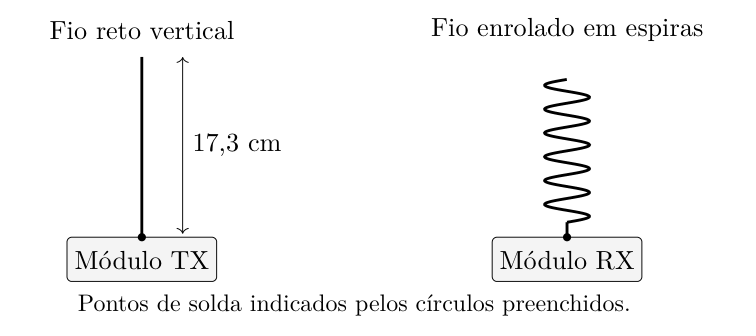
\includegraphics[width=\linewidth,height=135pt,keepaspectratio]{figuras/antenas.png}\caption{Geometria das antenas TX e RX, sem escala. Fonte: relatório técnico anterior.}\label{fig:antenas}\end{figure}
\subsubsection*{Dimensionamento do transmissor}
A antena TX foi confeccionada com comprimento de 17,3 cm, próximo de um quarto do comprimento de onda em espaço livre para 433 MHz:

\textbf{\ensuremath{\lambda} = c/f = 3,0 \ensuremath{\times} 10\textsuperscript{8} / (433 \ensuremath{\times} 10\textsuperscript{6}) \ensuremath{\approx} 0,693 m\\ L = \ensuremath{\lambda}/4 \ensuremath{\approx} 0,173 m = 17,3 cm.}

A antena RX helicoidal reduz a extensão física do fio. O diâmetro, o passo, o comprimento total e a quantidade de espiras não foram padronizados; por isso, não é possível determinar sua ressonância ou ganho a partir das fotos.

\begin{figure}[H]\centering
\begin{minipage}[t]{0.48\linewidth}\centering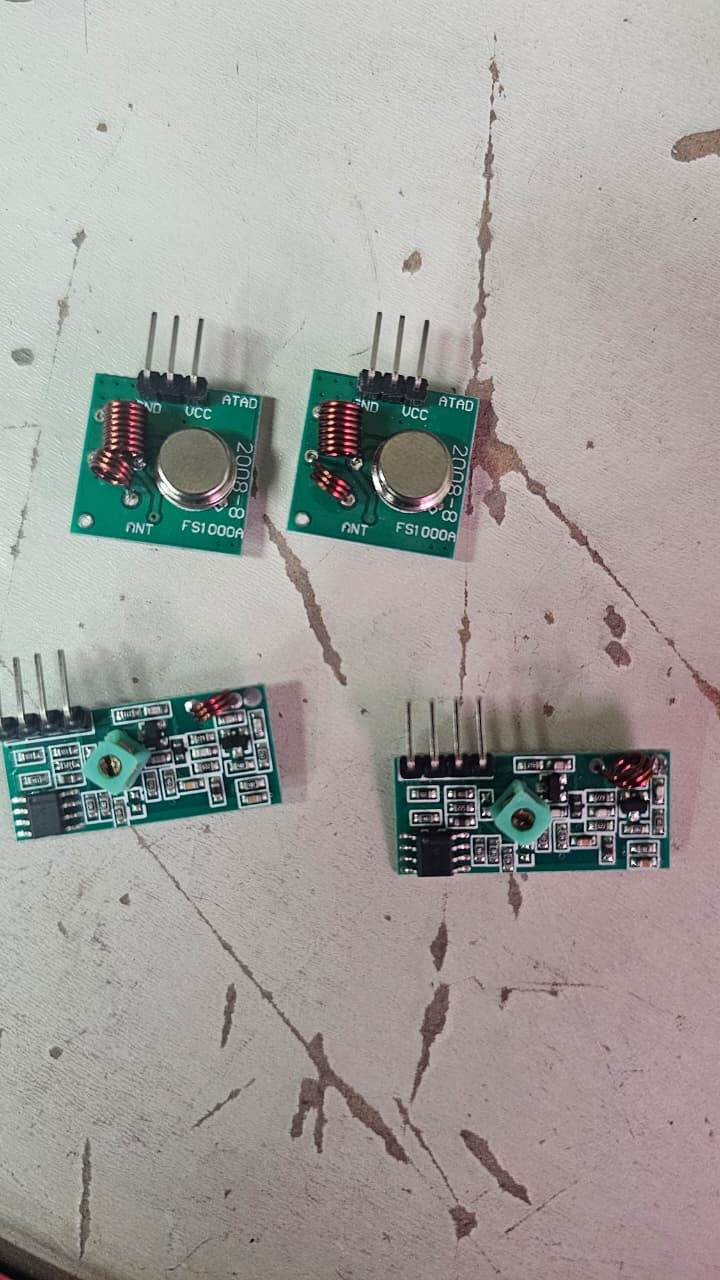
\includegraphics[width=\linewidth,height=150pt,keepaspectratio]{figuras/old_6_1.jpg}\caption{Conjuntos TX/RX utilizados.}\label{fig:old_6_1}\end{minipage}
\hfill
\begin{minipage}[t]{0.48\linewidth}\centering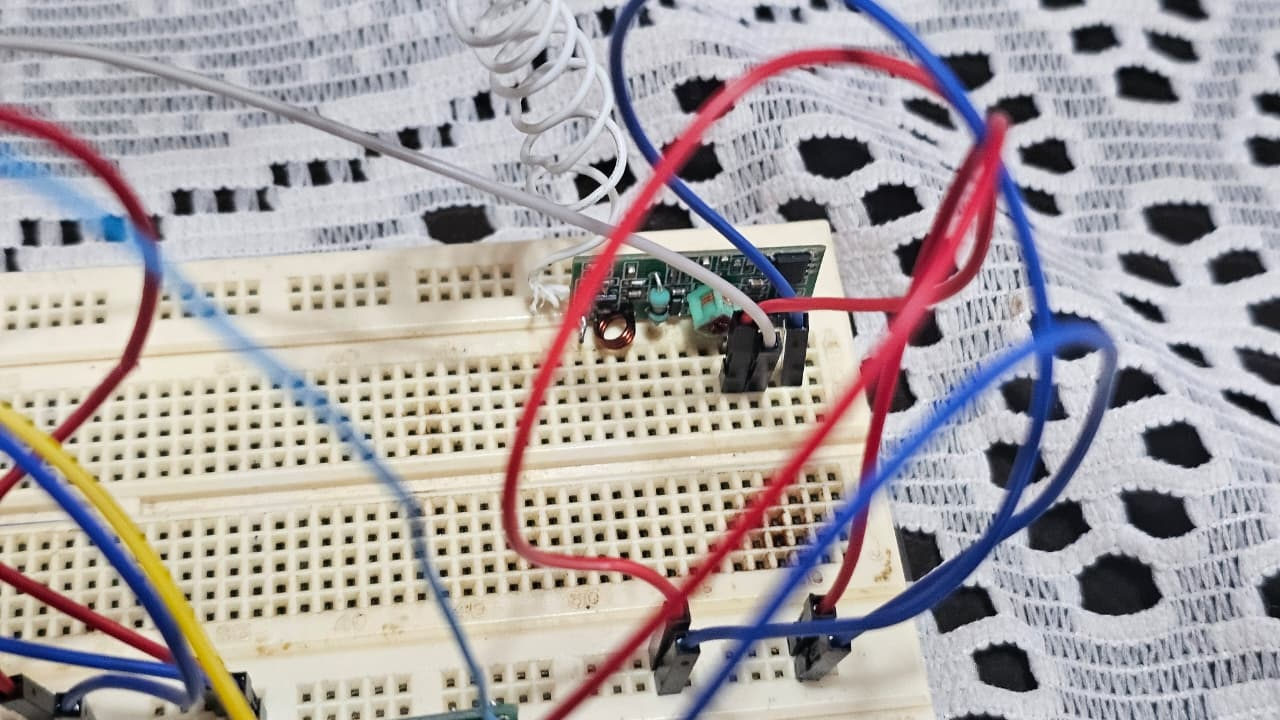
\includegraphics[width=\linewidth,height=150pt,keepaspectratio]{figuras/old_7_1.jpg}\caption{Detalhe da antena RX helicoidal.}\label{fig:old_7_1}\end{minipage}
\end{figure}
{\small Fonte das fotografias: acervo da equipe (2026). Não foram medidos impedância, ganho ou largura de banda. A montagem e a orientação das antenas influenciam o resultado do enlace.\par}
\setcounter{subsection}{2}\subsection{Circuito A — montagem}
\begin{figure}[H]
\centering
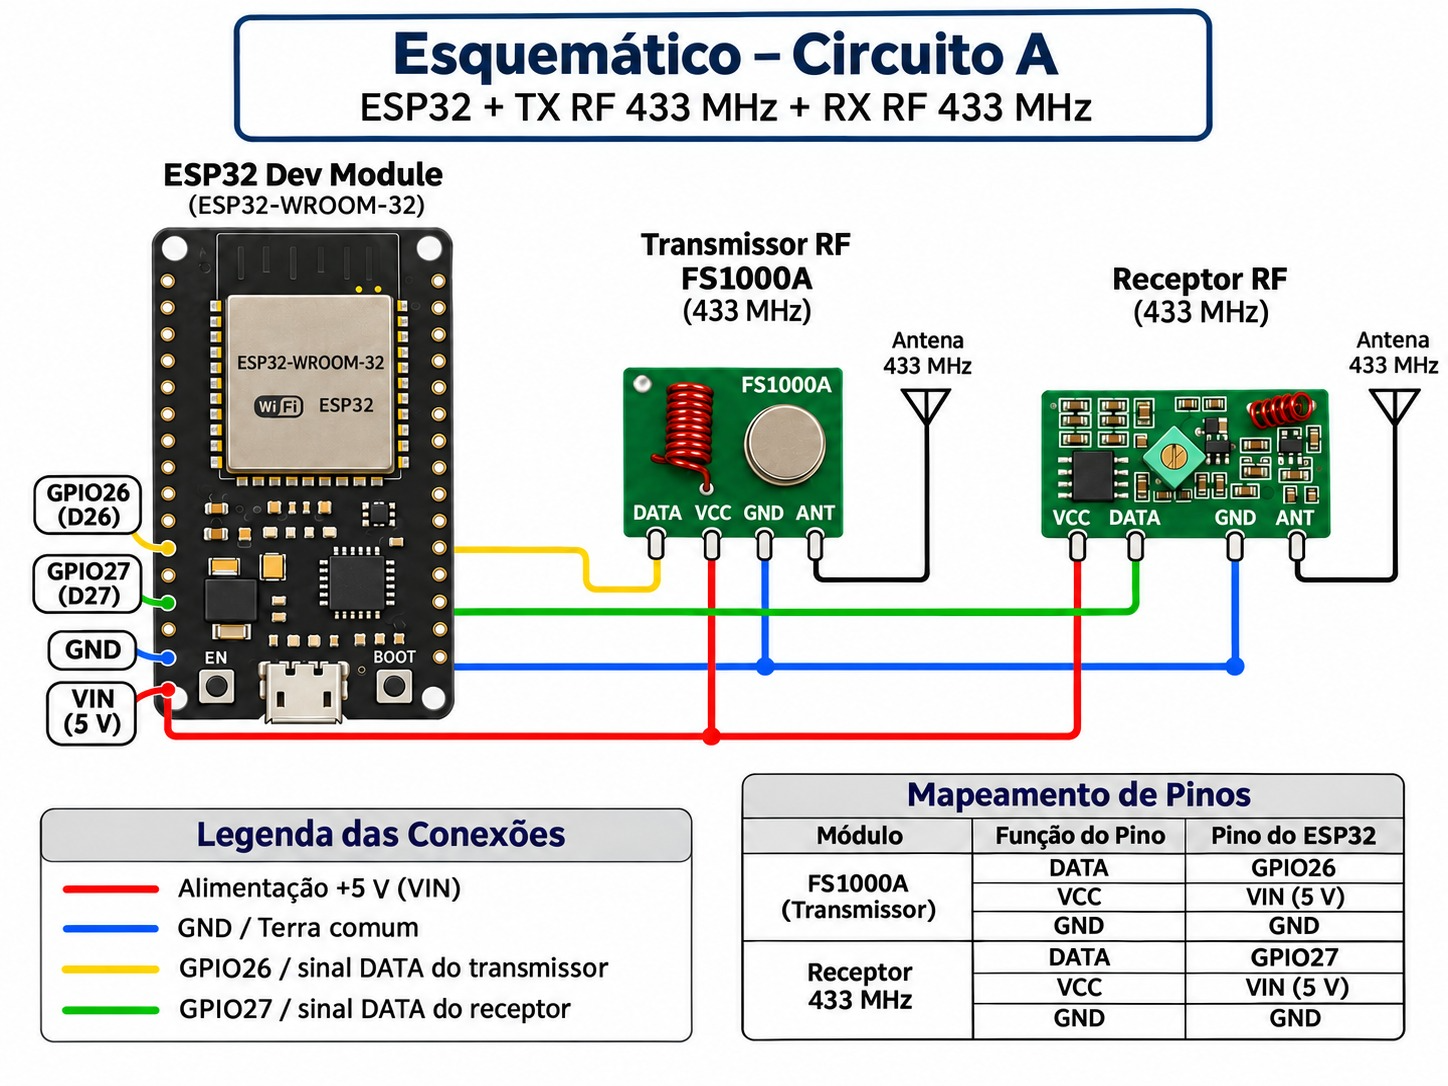
\includegraphics[width=\linewidth,height=225pt,keepaspectratio]{figuras/esq_a.png}
\caption{Esquemático atualizado do Circuito A (ESP32 + transmissor RF 433 MHz + receptor RF 433 MHz). Fonte: elaboração da equipe.}
\label{fig:esq_a}
\end{figure}
\begin{table}[H]\centering\small\caption{Mapeamento das ligações do circuito A}\label{tab:3}
\rowcolors{2}{tcdlight}{white}\begin{tabularx}{\linewidth}{>{\hsize=0.6186\hsize\linewidth=\hsize\raggedright\arraybackslash}X>{\hsize=1.3814\hsize\linewidth=\hsize\raggedright\arraybackslash}X}
\rowcolor{tcdnavy} \textcolor{white}{\textbf{Pino ESP32 A}} & \textcolor{white}{\textbf{Conexão}} \\
GPIO26 & DATA do transmissor RF. \\
GPIO27 & DATA do receptor RF (verificar nível lógico). \\
GND & Terra comum local, TX e RX. \\
Alimentação RF & Conforme tensão nominal dos módulos; verificar VIN/\allowbreak 5 V. \\
\bottomrule\end{tabularx}\end{table}
\begin{enumerate}
\item Posicionar o ESP32 e os módulos TX/RX na protoboard e conectar os terras locais.
\item Soldar as antenas com a montagem desenergizada. Interligar DATA TX ao GPIO26 e DATA RX ao GPIO27.
\item Conferir alimentação e níveis lógicos antes de energizar. Ligar o computador A ao ESP32 por USB.
\end{enumerate}
\begin{figure}[H]\centering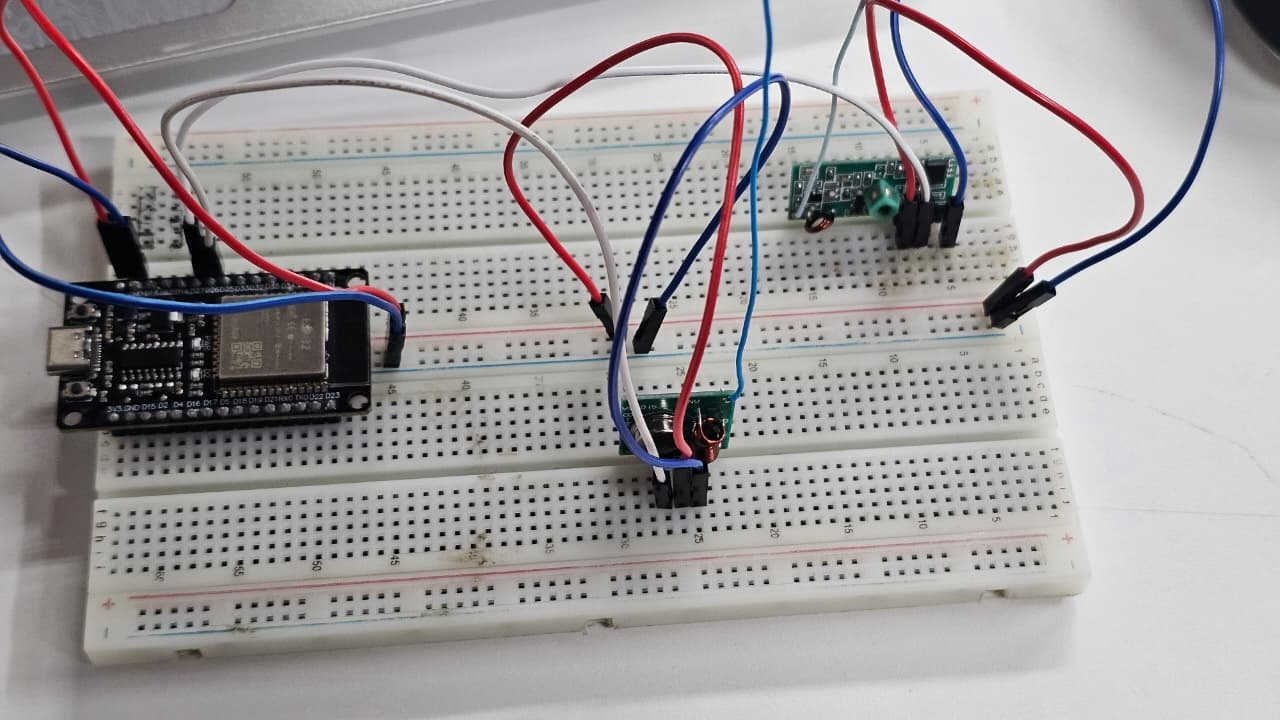
\includegraphics[width=\linewidth,height=180pt,keepaspectratio]{figuras/old_9_1.jpg}\caption{Montagem física do circuito A. Fonte: acervo da equipe.}\label{fig:old_9_1}\end{figure}
\setcounter{subsection}{3}\subsection{Circuito B — montagem}
\begin{figure}[H]
\centering
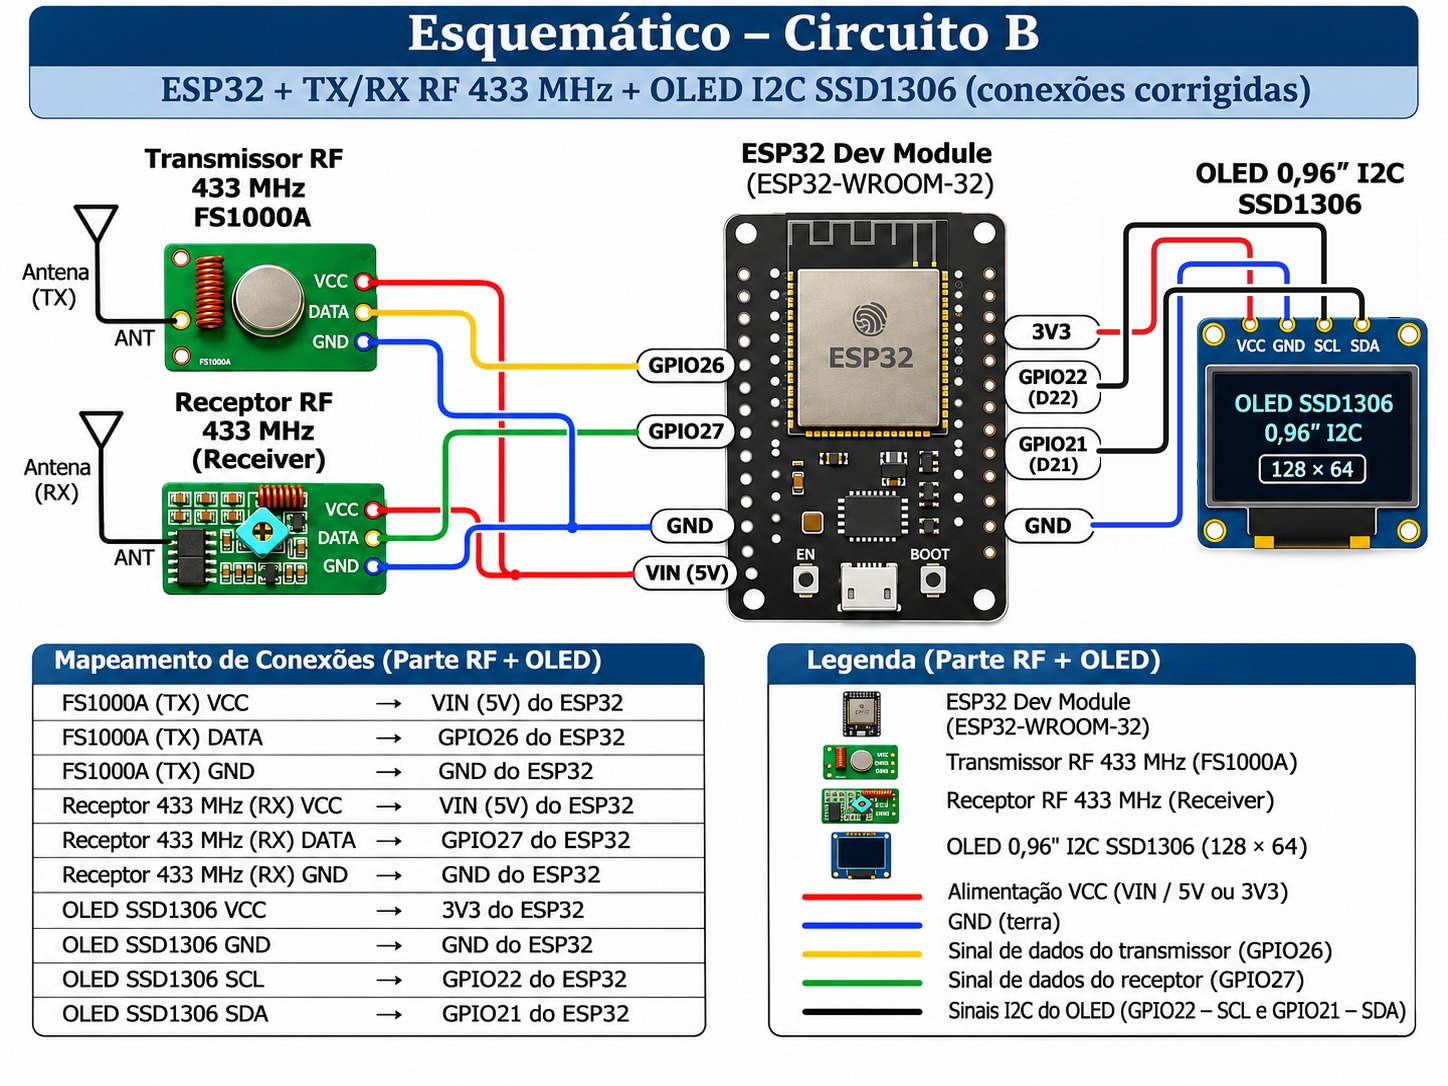
\includegraphics[width=\linewidth,height=225pt,keepaspectratio]{figuras/esq_b.png}
\caption{Esquemático atualizado do Circuito B, incluindo ESP32, módulos RF 433 MHz e display OLED SSD1306 com conexões corrigidas. Fonte: elaboração da equipe.}
\label{fig:esq_b}
\end{figure}
\begin{table}[H]\centering\small\caption{Mapeamento das ligações do circuito B}\label{tab:4}
\rowcolors{2}{tcdlight}{white}\begin{tabularx}{\linewidth}{>{\hsize=0.6186\hsize\linewidth=\hsize\raggedright\arraybackslash}X>{\hsize=1.3814\hsize\linewidth=\hsize\raggedright\arraybackslash}X}
\rowcolor{tcdnavy} \textcolor{white}{\textbf{Pino ESP32 B}} & \textcolor{white}{\textbf{Conexão}} \\
GPIO26 /\allowbreak  GPIO27 & DATA TX /\allowbreak  DATA RX, respectivamente. \\
GND & Terra comum local para TX, RX e OLED. \\
Alimentação RF & Conferir tensão e nível lógico do receptor. \\
GPIO21 /\allowbreak  GPIO22 & SDA /\allowbreak  SCL do OLED (I\textsuperscript{2}C). \\
3V3 & VCC do OLED SSD1306. \\
\bottomrule\end{tabularx}\end{table}
Repetir a montagem RF do circuito A. Acrescentar o display no barramento I\textsuperscript{2}C, alimentar o OLED em 3,3 V e ligar GND ao terra local. Conferir a ordem real dos pinos no módulo. O painel utilizado apresenta áreas amarela e azul, mas a imagem é monocromática em nível lógico.

\begin{figure}[H]\centering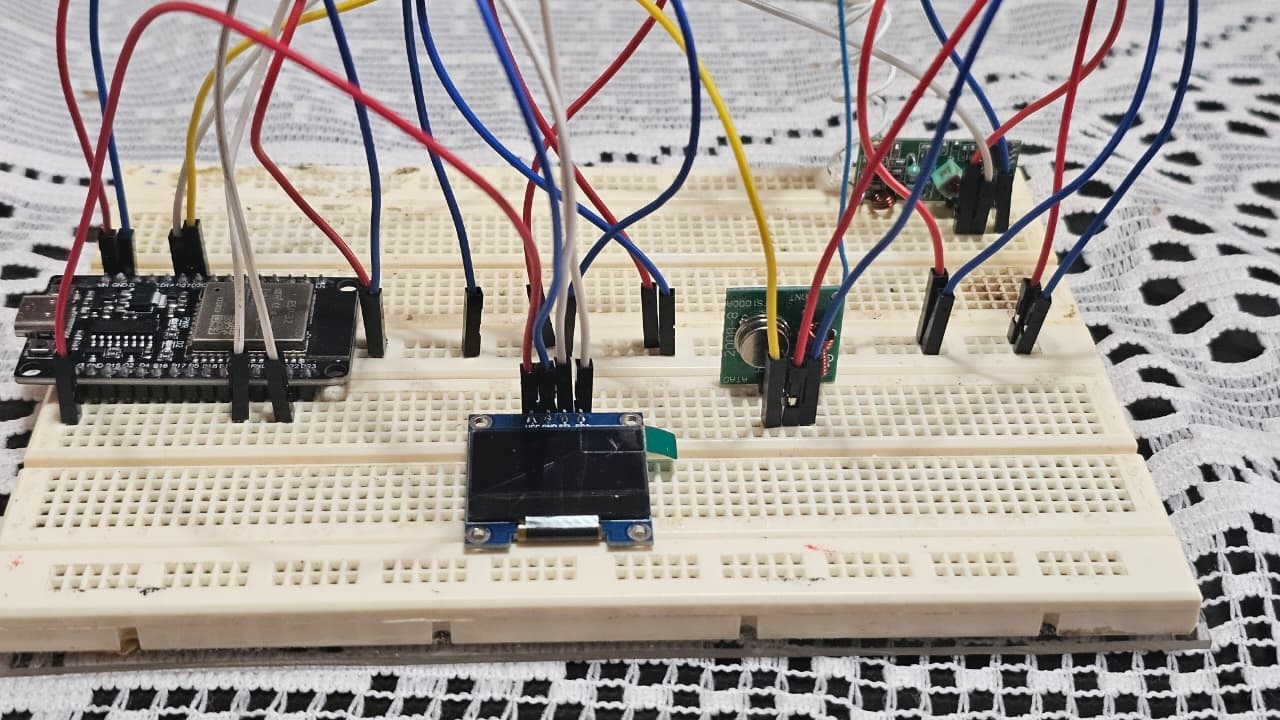
\includegraphics[width=\linewidth,height=180pt,keepaspectratio]{figuras/old_10_1.jpg}\caption{Montagem física de B com display OLED. Fonte: acervo da equipe.}\label{fig:old_10_1}\end{figure}

\clearpage\section{Ambiente de desenvolvimento}
A implementação utiliza dois sketches Arduino/C++ e dois scripts Python. A revisão V7 é a referência de validação; a variante V7R foi experimental e não deve ser misturada com ela. O README registra o core ESP32 2.0.17 como ambiente de compilação de referência, sem exigir que seja a única versão compatível.

\begin{table}[H]\centering\small\caption{Arquivos de implementação e suas funções}\label{tab:5}
\rowcolors{2}{tcdlight}{white}\begin{tabularx}{\linewidth}{>{\hsize=1.0309\hsize\linewidth=\hsize\raggedright\arraybackslash}X>{\hsize=0.9691\hsize\linewidth=\hsize\raggedright\arraybackslash}X}
\rowcolor{tcdtablehead} \textcolor{black}{\textbf{Arquivo no GitHub}} & \textcolor{black}{\textbf{Função}} \\
firmware/\allowbreak CircuitoA/\allowbreak CircuitoA.ino & Firmware do nó A. \\
firmware/\allowbreak CircuitoB/\allowbreak CircuitoB.ino & Firmware do nó B e display. \\
computador/\allowbreak enviar\_{}\allowbreak imagem\_{}\allowbreak TCD.py & Conversão e envio serial de pixels. \\
computador/\allowbreak receber\_{}\allowbreak imagem\_{}\allowbreak TCD.py & Recepção, validação e reconstrução. \\
computador/\allowbreak requirements.txt & Dependências dos scripts. \\
\bottomrule\end{tabularx}\end{table}
\setcounter{subsection}{0}\subsection{Instalação e gravação}
\begin{enumerate}
\item Instalar Arduino IDE e o suporte de placas ESP32 da Espressif Systems. Selecionar ESP32 Dev Module e a porta COM correspondente.
\item Para o circuito B, instalar as bibliotecas Adafruit SSD1306, Adafruit GFX e Adafruit BusIO. A interface I\textsuperscript{2}C utiliza Wire.
\item Abrir o sketch A, compilar e gravar no ESP32 A. Repetir no ESP32 B com o sketch B. Conferir a versão V7 no terminal de inicialização.
\item Abrir os dois Monitores Seriais em 115200 baud, com final de linha “Nova linha”. Executar /teste nos dois nós.
\item Instalar Python e dependências. Para transferências de imagens, fechar os Monitores Seriais antes de abrir as portas com os scripts.
\end{enumerate}
\par\noindent\begin{minipage}{\linewidth}
\begin{lstlisting}
python -m pip install pyserial pillow
python -m serial.tools.list_ports
\end{lstlisting}
\end{minipage}\par
{\small As portas COM variaram durante o projeto. Em T12–T13, foram A COM20 e B COM8; em T14, A COM20 e B COM5. Sempre conferir as portas atuais.\par}
\setcounter{subsection}{1}\subsection{Fluxo de execução e comandos}
O firmware trata os comandos locais do Monitor Serial e os dados recebidos pelo rádio. O texto comum é convertido em bytes, fragmentado em blocos de até 16 bytes e transmitido quadro a quadro. O circuito remoto acumula apenas os blocos novos até o END. O contador de sequência alternado evita anexar a mesma carga útil novamente.

\begin{table}[H]\centering\small\caption{Comandos do Monitor Serial}\label{tab:6}
\rowcolors{2}{tcdlight}{white}\begin{tabularx}{\linewidth}{>{\hsize=0.5278\hsize\linewidth=\hsize\raggedright\arraybackslash}X>{\hsize=1.4722\hsize\linewidth=\hsize\raggedright\arraybackslash}X}
\rowcolor{tcdtablehead} \textcolor{black}{\textbf{Comando}} & \textcolor{black}{\textbf{Uso}} \\
/\allowbreak ajuda & Listar comandos disponíveis. \\
/\allowbreak teste & Verificar CRC-8 e 4B6B localmente. \\
/\allowbreak status & Exibir contadores acumulados. \\
/\allowbreak zerarstats & Zerar contadores sem reiniciar sequência ou protocolo. \\
/\allowbreak erro & Corromper um bit na próxima tentativa de DATA. \\
/\allowbreak ruido N & Induzir N corrupções por software. \\
/\allowbreak perderack & Omitir uma confirmação DATA. \\
/\allowbreak perderend & Omitir uma confirmação END. \\
/\allowbreak lote N & Enviar N mensagens numeradas, de 1 a 30. \\
Texto comum & Enviar uma mensagem ao outro circuito. \\
\bottomrule\end{tabularx}\end{table}
\subsubsection*{Procedimento de envio de texto}
\begin{enumerate}
\item Aguardar a conclusão de toda sessão anterior. Executar /zerarstats nos dois monitores quando necessário.
\item Digitar o texto apenas no monitor do emissor. Observar as confirmações DATA e END.
\item Conferir TEXTO COMPLETO no receptor e a apresentação no OLED quando o destino for B. Registrar /status nos dois circuitos antes de zerar contadores.
\end{enumerate}
O comando /lote deve conter espaço antes do número. /zerarstats não redefine o estado de comunicação. Se a sessão não terminar, anotar os logs e reiniciar ambos os nós para recuperar uma sessão sincronizada, conforme o protocolo de ensaios.


\section{Implementação e análise dos códigos-fonte}
\label{sec:implementacao}
Os dois firmwares V7 originais (906 linhas cada) e os dois scripts Python estão disponíveis no repositório do projeto. Esta seção descreve os blocos que integram o firmware Arduino/C++ e os programas Python, sem reproduzir integralmente os códigos nem alterar a versão validada nos ensaios.

\subsection{Firmwares dos circuitos A e B}
Os dois sketches compartilham a mesma estrutura de comunicação. A constante de compilação \texttt{NO\_EH\_B} vale 0 no circuito A e 1 no circuito B, habilitando neste último as rotinas do OLED. Ambos utilizam GPIO26 para TX, GPIO27 para RX, UART RF a 1.200 baud e USB a 115.200 baud. Em \texttt{setup()}, o firmware inicializa a serial, o rádio e, no B, procura o endereço I\textsuperscript{2}C 0x3C ou 0x3D do display. Em \texttt{loop()}, lê comandos da USB e verifica se há quadros RF recebidos.

\begin{table}[H]\centering\small\caption{Principais funções dos firmwares V7}\label{tab:funcoes-firmware}
\rowcolors{2}{tcdlight}{white}\begin{tabularx}{\linewidth}{>{\raggedright\arraybackslash}p{0.43\linewidth}X}
\rowcolor{tcdtablehead}\textcolor{black}{\textbf{Funções}} & \textcolor{black}{\textbf{Responsabilidade}}\\
\texttt{setup(), loop(), lerUSB()} & Inicialização, leitura de comandos e atendimento do rádio.\\
\texttt{montarFrame(), crc8()} & Montagem do quadro de 21 bytes e cálculo do FCS.\\
\texttt{escrever4b6b(), dec4b6b()} & Conversão entre nibbles de 4 bits e símbolos de 6 bits.\\
\texttt{transmitirFrame(), receberFrame()} & Envio, enquadramento, decodificação e verificação dos quadros.\\
\texttt{enviarComARQ(), esperarACK()} & Retransmissão após timeout e validação da sequência do ACK.\\
\texttt{processarFrameRecebido()} & Controle de duplicatas, remontagem de texto/imagem e tratamento do END.\\
\texttt{iniciarEnvioImagem(), enviarBlocoImagem(), encerrarEnvioImagem()} & Transferência de cabeçalho, blocos de pixels e encerramento.\\
\texttt{mostrarImagemOLED(), exportarImagemParaUSB()} & Exibição no B e exportação dos dados validados ao computador.\\
\texttt{testeLocal(), imprimirStatus()} & Autoteste e registro dos contadores experimentais.\\
\bottomrule\end{tabularx}\end{table}

O trecho abaixo, extraído de \texttt{loop()} (linhas 895--906 dos sketches consultados), mostra o atendimento dos quadros válidos e o registro dos erros de recepção. A lógica de retransmissão fica em \texttt{enviarComARQ()}, que repete o quadro até obter ACK válido; a sequência só avança após confirmação. O tratamento de DATA e END duplicados impede a entrega repetida da mesma carga útil.
\par\noindent\begin{minipage}{\linewidth}
\begin{lstlisting}[language=C++,caption={Trecho original do laço principal do firmware V7},label={lst:loop-v7}]
void loop() {
  lerUSB();
  uint8_t f[TAM_FRAME] = {0};
  uint8_t r = receberFrame(f, 150);
  if (r == FRAME_OK) {
    ++stats.framesValidos;
    processarFrameRecebido(f);
  } else if (r != SEM_SINAL) {
    registrarErro(r);
  }
  delay(1);
}
\end{lstlisting}
\end{minipage}\par

\subsection{Programas Python de envio e recepção}
O script de envio utiliza Pillow [12] para corrigir orientação, redimensionar e converter a imagem para 1 bit por pixel. Calcula CRC32 e SHA-256 sobre os bytes dos pixels, salva o PBM de referência e utiliza PySerial [11] para transmitir os comandos \texttt{/imgstart}, \texttt{/imghex} e \texttt{/imgend}. Aguarda as respostas \texttt{@PC\_READY}, \texttt{@PC\_ACK} e \texttt{@PC\_DONE} antes de avançar. O bloco hexadecimal representa 16 bytes de pixels; o firmware realiza a transmissão RF e o controle ARQ.

No destino, o script de recepção utiliza a classe \texttt{Receptor} e sua função \texttt{processar()} para interpretar \texttt{@IMG\_BEGIN}, \texttt{@IMG\_DATA} e \texttt{@IMG\_END}. Acumula os bytes, confere o tamanho e o CRC32 antes de gravar o PBM e, quando Pillow está instalado, o PNG. O SHA-256 é impresso para comparação com o emissor; não é transmitido como campo do quadro RF. Assim, CRC-8 verifica cada quadro, CRC32 verifica a imagem completa e SHA-256 permite a conferência adicional dos pixels.

\noindent\textbf{Acesso aos códigos originais:} \href{https://github.com/enzogomes2006/tcd-rf433-esp32/blob/35d4604424820aa82c8c3423637b6a23ae0019b2/firmware/CircuitoA/CircuitoA.ino}{Circuito A} \textperiodcentered\ \href{https://github.com/enzogomes2006/tcd-rf433-esp32/blob/35d4604424820aa82c8c3423637b6a23ae0019b2/firmware/CircuitoB/CircuitoB.ino}{Circuito B} \textperiodcentered\ \href{https://github.com/enzogomes2006/tcd-rf433-esp32/blob/35d4604424820aa82c8c3423637b6a23ae0019b2/computador/enviar_imagem_TCD.py}{Python de envio} \textperiodcentered\ \href{https://github.com/enzogomes2006/tcd-rf433-esp32/blob/35d4604424820aa82c8c3423637b6a23ae0019b2/computador/receber_imagem_TCD.py}{Python de recepção}. A revisão de referência indicada no repositório é 35d4604; os arquivos foram consultados em 25/11/2026.

\clearpage\section{Protocolo de comunicação}
A UART Serial2 opera a 1200 baud, 8N1; a comunicação USB utiliza 115200 baud. A unidade lógica de transmissão possui 21 bytes, mesmo quando o campo DATA contém menos de 16 bytes úteis. Os bytes restantes são preenchidos com zero.

\begin{table}[H]\centering\small\caption{Estrutura do quadro lógico}\label{tab:7}
\rowcolors{2}{tcdlight}{white}\begin{tabularx}{\linewidth}{>{\hsize=0.7010\hsize\linewidth=\hsize\raggedright\arraybackslash}X>{\hsize=0.6186\hsize\linewidth=\hsize\raggedright\arraybackslash}X>{\hsize=0.4536\hsize\linewidth=\hsize\raggedright\arraybackslash}X>{\hsize=2.2268\hsize\linewidth=\hsize\raggedright\arraybackslash}X}
\rowcolor{tcdnavy} \textcolor{white}{\textbf{Campo}} & \textcolor{white}{\textbf{Posição}} & \textcolor{white}{\textbf{Bytes}} & \textcolor{white}{\textbf{Função}} \\
FLAG & 0 & 1 & 0x7E; início do quadro. \\
TYPE & 1 & 1 & DATA=0; ACK=1; END=2. \\
SEQ & 2 & 1 & Sequência alternada 0 ou 1. \\
LEN & 3 & 1 & Comprimento útil de DATA. \\
DATA & 4–19 & 16 & Dados e preenchimento. \\
FCS & 20 & 1 & CRC-8 sobre TYPE, SEQ, LEN e DATA. \\
\bottomrule\end{tabularx}\end{table}
\setcounter{subsection}{0}\subsection{Enquadramento e estados}
DATA transporta a carga útil. ACK confirma a recepção de um quadro válido e deve corresponder ao número de sequência esperado. END delimita a sessão e também exige ACK. O transmissor só avança após a confirmação; o receptor utiliza a sequência para identificar uma repetição.

\begin{table}[H]\centering\small\caption{Parâmetros de referência do firmware V7}\label{tab:8}
\rowcolors{2}{tcdlight}{white}\begin{tabularx}{\linewidth}{>{\hsize=1.0722\hsize\linewidth=\hsize\raggedright\arraybackslash}X>{\hsize=0.9278\hsize\linewidth=\hsize\raggedright\arraybackslash}X}
\rowcolor{tcdnavy} \textcolor{white}{\textbf{Parâmetro de referência V7}} & \textcolor{white}{\textbf{Valor}} \\
Preâmbulo & 32 bytes lógicos 0x2A, codificados em 4B6B. \\
Quadro lógico /\allowbreak  payload & 21 bytes /\allowbreak  até 16 bytes. \\
Timeout ACK /\allowbreak  leitura de quadro & 5000 ms /\allowbreak  1600 ms. \\
Espera antes do ACK /\allowbreak  intervalo entre cópias & 180 ms /\allowbreak  35 ms. \\
Cópias de ACK /\allowbreak  pausa após ACK válido & 2 /\allowbreak  1200 ms. \\
Limite de reenvios & Sem limite no firmware. \\
Buffer texto /\allowbreak  imagem & 512 /\allowbreak  1024 bytes. \\
\bottomrule\end{tabularx}\end{table}
Esses parâmetros correspondem à documentação V7. A pausa, as cópias de ACK e o preâmbulo aumentam a duração da transferência, mas buscam reduzir problemas observados no enlace RF.

\setcounter{subsection}{1}\subsection{Cálculo do FCS por CRC-8}
O FCS (Frame Check Sequence) é calculado pelo polinômio CRC-8 0x87, equivalente a x\textsuperscript{8} + x\textsuperscript{7} + x\textsuperscript{2} + x + 1, com registrador inicial 0x00, sem reflexão e sem XOR final. O cálculo inclui os 19 bytes de TYPE, SEQ, LEN e DATA. FLAG e o próprio FCS não entram no cálculo.

\par\noindent\begin{minipage}{\linewidth}
\begin{lstlisting}
uint8_t crc8(const uint8_t *dados, size_t n) {
  uint8_t crc = 0;
  for (size_t i = 0; i < n; ++i) {
    crc ^= dados[i];
    for (uint8_t b = 0; b < 8; ++b)
      crc = (crc & 0x80) ? (uint8_t)((crc << 1) ^ 0x87)
                        : (uint8_t)(crc << 1);
  }
  return crc;
}
\end{lstlisting}
\end{minipage}\par
\subsubsection*{Exemplo: mensagem ASCII TCD}
TYPE=00, SEQ=00, LEN=03. Os bytes úteis são 54 43 44; completam-se os 16 bytes de DATA com 13 zeros. O registrador é atualizado a cada byte.

\begin{table}[H]\centering\small\caption{Estados intermediários do CRC-8}\label{tab:9}
\rowcolors{2}{tcdlight}{white}\begin{tabularx}{\linewidth}{>{\hsize=0.7423\hsize\linewidth=\hsize\raggedright\arraybackslash}X>{\hsize=1.2577\hsize\linewidth=\hsize\raggedright\arraybackslash}X}
\rowcolor{tcdnavy} \textcolor{white}{\textbf{Entrada (hexadecimal)}} & \textcolor{white}{\textbf{CRC após cada byte (hexadecimal)}} \\
00 00 03 54 43 44 & 00 00 0E 83 8E AA \\
13 bytes 00 & ED 0C 38 4D C5 9C 11 5A 83 FA 4A 5E 16 \\
\bottomrule\end{tabularx}\end{table}
\textbf{FCS calculado: 0x16.} Se o byte 0x54 for alterado para 0x55 sem recalcular o FCS, o receptor calcula 0x22 e rejeita o quadro. A ausência de ACK aciona a retransmissão pelo ARQ.

\par\noindent\begin{minipage}{\linewidth}
\begin{lstlisting}
7E 00 00 03 54 43 44 00 00 00 00
00 00 00 00 00 00 00 00 00 16
\end{lstlisting}
\end{minipage}\par
O CRC detecta corrupção, mas não corrige o dado diretamente nem garante detecção de todos os padrões de erro possíveis. A recuperação depende da retransmissão.

\setcounter{subsection}{2}\subsection{Codificação 4B6B e ARQ}
Cada byte lógico é dividido em dois nibbles. Cada nibble de quatro bits é mapeado em um símbolo de seis bits, transportado em um caractere UART de oito bits. Símbolos inválidos são rejeitados antes da verificação do CRC.

\begin{table}[H]\centering\small\caption{Tabela de codificação 4B6B}\label{tab:10}
\rowcolors{2}{tcdlight}{white}\begin{tabularx}{\linewidth}{>{\hsize=1.5773\hsize\linewidth=\hsize\raggedright\arraybackslash}X>{\hsize=0.9278\hsize\linewidth=\hsize\raggedright\arraybackslash}X>{\hsize=0.9278\hsize\linewidth=\hsize\raggedright\arraybackslash}X>{\hsize=0.9278\hsize\linewidth=\hsize\raggedright\arraybackslash}X>{\hsize=0.9278\hsize\linewidth=\hsize\raggedright\arraybackslash}X>{\hsize=0.9278\hsize\linewidth=\hsize\raggedright\arraybackslash}X>{\hsize=0.9278\hsize\linewidth=\hsize\raggedright\arraybackslash}X>{\hsize=0.9278\hsize\linewidth=\hsize\raggedright\arraybackslash}X>{\hsize=0.9278\hsize\linewidth=\hsize\raggedright\arraybackslash}X}
\rowcolor{tcdnavy} \textcolor{white}{\textbf{Nibble}} & \textcolor{white}{\textbf{0}} & \textcolor{white}{\textbf{1}} & \textcolor{white}{\textbf{2}} & \textcolor{white}{\textbf{3}} & \textcolor{white}{\textbf{4}} & \textcolor{white}{\textbf{5}} & \textcolor{white}{\textbf{6}} & \textcolor{white}{\textbf{7}} \\
Símbolo & 0D & 0E & 13 & 15 & 16 & 19 & 1A & 1C \\
Nibble & 8 & 9 & A & B & C & D & E & F \\
Símbolo & 23 & 25 & 26 & 29 & 2A & 2C & 32 & 34 \\
\bottomrule\end{tabularx}\end{table}
O preâmbulo de 32 bytes e o quadro de 21 bytes resultam em (32 + 21) \ensuremath{\times} 2 = 106 caracteres UART. Em 8N1, cada caractere ocupa 10 bits, totalizando 1.060 bits por transmissão. A 1200 baud, a serialização teórica é de aproximadamente 0,883 s, sem considerar ACKs, pausas, processamento e reenvios.

\subsubsection*{Stop-and-Wait ARQ: sequência alternada}
\begin{table}[H]\centering\small\caption{Sequência de transmissão e confirmação}\label{tab:11}
\rowcolors{2}{tcdlight}{white}\begin{tabularx}{\linewidth}{>{\hsize=0.9979\hsize\linewidth=\hsize\raggedright\arraybackslash}X>{\hsize=1.0021\hsize\linewidth=\hsize\raggedright\arraybackslash}X}
\rowcolor{tcdnavy} \textcolor{white}{\textbf{Emissor}} & \textcolor{white}{\textbf{Receptor}} \\
Envia DATA seq=0 e aguarda. & Valida CRC, aceita DATA e envia ACK seq=0. \\
ACK perdido: após timeout, reenvia DATA seq=0. & Identifica duplicata, não concatena e reenvia ACK. \\
Recebe ACK válido, alterna sequência. & Espera próximo quadro novo. \\
Envia DATA seq=1 ou END com a sequência aplicável. & Valida, confirma; END delimita a sessão. \\
\bottomrule\end{tabularx}\end{table}
O receptor confirma novamente duplicatas sem acrescentar os bytes uma segunda vez. Após END aceito, um END repetido não entrega uma nova mensagem. O firmware coloca o sinal TX em LOW ao retornar à recepção; isso não significa necessariamente desligar a alimentação do módulo. O limite de tentativas é indefinido, o que exige intervenção caso a comunicação não se restabeleça.


\clearpage\section{Transmissão e reconstrução de imagens}
O script transmissor lê uma imagem, corrige a orientação EXIF, converte para cinza, redimensiona preservando proporção, centraliza em fundo branco, inverte e converte para um bit por pixel. O dithering Floyd–Steinberg pode ser desativado com --sem-dither. O conteúdo transportado é o bitmap resultante, não os bytes do JPEG original.

\begin{table}[H]\centering\small\caption{Estrutura do cabeçalho de imagem}\label{tab:12}
\rowcolors{2}{tcdlight}{white}\begin{tabularx}{\linewidth}{>{\hsize=1.5052\hsize\linewidth=\hsize\raggedright\arraybackslash}X>{\hsize=0.4948\hsize\linewidth=\hsize\raggedright\arraybackslash}X}
\rowcolor{tcdnavy} \textcolor{white}{\textbf{Campo do cabeçalho TCDIM1}} & \textcolor{white}{\textbf{Bytes}} \\
Identificador ASCII TCDIM1 & 6 \\
Largura e altura & 1 + 1 \\
Total de bytes de pixels (uint16 LE) & 2 \\
CRC32 (uint32 LE) & 4 \\
Reservados & 2 \\
\bottomrule\end{tabularx}\end{table}
\begin{table}[H]\centering\small\caption{Quantidade de bytes e quadros por resolução}\label{tab:13}
\rowcolors{2}{tcdlight}{white}\begin{tabularx}{\linewidth}{>{\hsize=0.8660\hsize\linewidth=\hsize\raggedright\arraybackslash}X>{\hsize=1.0309\hsize\linewidth=\hsize\raggedright\arraybackslash}X>{\hsize=1.0309\hsize\linewidth=\hsize\raggedright\arraybackslash}X>{\hsize=1.0722\hsize\linewidth=\hsize\raggedright\arraybackslash}X}
\rowcolor{tcdnavy} \textcolor{white}{\textbf{Resolução}} & \textcolor{white}{\textbf{Bytes de pixels}} & \textcolor{white}{\textbf{DATA de pixels}} & \textcolor{white}{\textbf{Quadros lógicos\textsuperscript{1}}} \\
64\ensuremath{\times}32 & 256 & 16 & 18 \\
128\ensuremath{\times}64 & 1024 & 64 & 66 \\
\bottomrule\end{tabularx}\end{table}
{\small \textsuperscript{1} Inclui um DATA de metadados e um END, sem ACKs ou reenvios.\par}
O receptor acumula os bytes em ordem, verifica tamanho e CRC32, confirma END e exporta o conteúdo por USB. O script receptor grava PBM e PNG e calcula SHA-256 dos bytes de pixels. O SHA-256 deve coincidir entre emissor e receptor do mesmo ensaio; não se compara o hash do JPEG original com o do bitmap convertido. O CRC32 usa polinômio refletido 0xEDB88320, inicialização e XOR final 0xFFFFFFFF.

\begin{figure}[H]\centering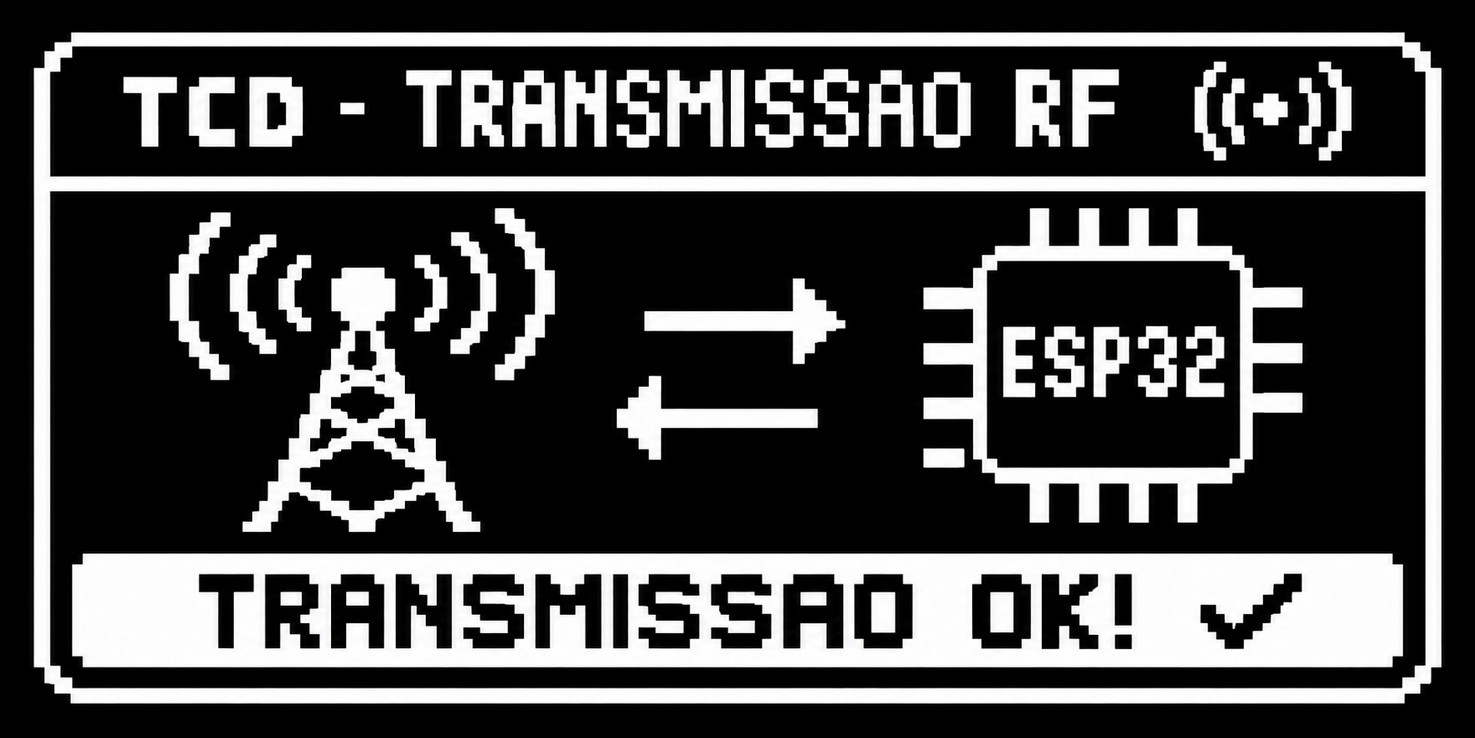
\includegraphics[width=\linewidth,height=145pt,keepaspectratio]{figuras/new_17_1.jpg}\caption{Imagem JPEG de referência utilizada nos ensaios. Fonte: relatório de ensaios, figura 28.}\label{fig:new_17_1}\end{figure}
\setcounter{subsection}{0}\subsection{Passo a passo da transmissão de imagem}
\begin{enumerate}
\item Preparar imagem4.jpeg na pasta em que o script transmissor será executado. Instalar pyserial e Pillow nos dois computadores.
\item Fechar os Monitores Seriais. Conferir a COM atribuída a cada ESP32; uma porta serial não pode ser usada simultaneamente pelo Arduino IDE e pelo script Python.
\item Abrir primeiro o receptor no computador de destino. Para T12 e T13, o receptor foi o B, na COM8.
\item Executar o transmissor no computador de origem. A opção --size seleciona 64\ensuremath{\times}32 ou 128\ensuremath{\times}64. Aguardar a confirmação completa, inclusive END.
\item No destino, conferir o total de bytes, CRC32 e SHA-256 dos pixels. Abrir o PBM/PNG e observar o OLED se o destino for B.
\item Encerrar o receptor antes de inverter o sentido. No T14, A recebeu na COM20 e B enviou pela COM5.
\end{enumerate}
\par\noindent\begin{minipage}{\linewidth}
\begin{lstlisting}
# Receptor B (T12 e T13)
python receber_imagem_TCD.py COM8

# Transmissor A: executar uma resolução por sessão
python enviar_imagem_TCD.py COM20 "imagem4.jpeg" --size 64x32
python enviar_imagem_TCD.py COM20 "imagem4.jpeg" --size 128x64
\end{lstlisting}
\end{minipage}\par
\par\noindent\begin{minipage}{\linewidth}
\begin{lstlisting}
# T14: receptor A; depois transmissor B
python receber_imagem_TCD.py COM20
py enviar_imagem_TCD.py COM5 "imagem4.jpeg" --size 64x32
\end{lstlisting}
\end{minipage}\par
\subsubsection*{Tratamento de falhas observadas}
Se houver erro de acesso à porta COM, fechar programas que a utilizam, verificar o cabo e identificar novamente a porta. Se ocorrerem timeouts sucessivos, registrar o log, encerrar a sessão e diagnosticar primeiro por texto. No T12 houve ClearCommError depois da validação e do salvamento; no T14, a primeira sessão foi interrompida e o envio foi retomado após diagnóstico. Não interpretar uma tentativa interrompida como uma transferência bem-sucedida.


\clearpage\section{Metodologia e resultados experimentais}
Foram definidos 14 ensaios no protocolo de 23/11/2026. Nos T01–T11, o Monitor Serial foi utilizado para comandos e contadores; nos T12–T14, os scripts Python transferiram imagens. A consolidação de 24/11/2026 distingue resultado relatado, comprovação parcial, sucesso funcional e integridade confirmada. As evidências dos T01–T09 presentes no relatório anterior complementam a revisão recente.

\begin{table}[H]\centering\small\caption{ID / Ensaio / Resultado / classificação}\label{tab:14}
\rowcolors{2}{tcdlight}{white}\begin{tabularx}{\linewidth}{>{\hsize=0.3093\hsize\linewidth=\hsize\raggedright\arraybackslash}X>{\hsize=1.0825\hsize\linewidth=\hsize\raggedright\arraybackslash}X>{\hsize=1.6082\hsize\linewidth=\hsize\raggedright\arraybackslash}X}
\rowcolor{tcdtablehead} \textcolor{black}{\textbf{ID}} & \textcolor{black}{\textbf{Ensaio}} & \textcolor{black}{\textbf{Resultado /\allowbreak  classificação}} \\
T01 & Autoteste CRC-8 e 4B6B & Três verificações OK; relatado. \\
T02 & Texto A \ensuremath{\to} B & Entrega e END; relatado. \\
T03 & Texto B \ensuremath{\to} A & Entrega; 2 reenvios; relatado. \\
T04 & Fragmentação & Entrega; 18 reenvios; relatado. \\
T05 & Corrupção CRC-8 & 1 CRC errado; recuperação; relatado. \\
T06 & Três erros simulados & 3 CRC errados; 1 mensagem; parcial. \\
T07 & Perda ACK DATA & Omissão, repetição e entrega; relatado. \\
T08 & Perda ACK END & END na terceira tentativa; relatado. \\
T09 & Lote curto & 10 recebidas; contadores residuais. \\
T10 & Distância >1 m & 10/\allowbreak 10, 1,12 m; funcional. \\
T11 & Obstáculo passivo & 10/\allowbreak 10 em cada condição; funcional. \\
T12 & Imagem A \ensuremath{\to} B, 64\ensuremath{\times}32 & 256 bytes; hashes iguais; íntegra. \\
T13 & Imagem A \ensuremath{\to} B, 128\ensuremath{\times}64 & 1024 bytes; hashes iguais; íntegra. \\
T14 & Imagem B \ensuremath{\to} A, 64\ensuremath{\times}32 & 256 bytes; hashes iguais; íntegra. \\
\bottomrule\end{tabularx}\end{table}
{\small Critérios transversais: conteúdo correto, número de sequência e END confirmado; em imagens, tamanho, CRC32 e SHA-256 dos pixels. A execução dos 14 ensaios não equivale à aprovação formal de todos os critérios. NR = não registrado.\par}
\setcounter{subsection}{0}\subsection{T01 a T05 — texto e detecção de erros}
\subsubsection*{T01 — Autoteste local}
Executar /teste em A e B. Os registros anteriores indicam CRC=OK, detecção de alteração=OK e 4B6B=OK nos dois nós. Este teste é local e não mede alcance RF.

\subsubsection*{T02 — Texto de A para B}
Zerar contadores, enviar TCD TESTE A PARA B em A e consultar /status nos dois circuitos. O relatório anterior registra texto completo em B e END confirmado em A. A OLED deve apresentar o texto; a fotografia específica não consta da consolidação atual.

\subsubsection*{T03 — Texto de B para A}
Zerar contadores, enviar TCD RESPOSTA B PARA A em B e consultar /status. Foram registrados 5 TX, 3 ACKs e 2 reenvios em B; A contabilizou uma mensagem, sem CRC errado ou duplicatas.

\subsubsection*{T04 — Fragmentação}
Enviar TESTE DE TEXTO LONGO - PACOTES DE 16 BYTES - TCD 2026 a partir de A. A mensagem de 53 bytes foi remontada em B, em quatro DATA (16+16+16+5) e END. A registrou 23 TX, 5 ACKs e 18 reenvios; B registrou 18 duplicatas e uma mensagem. A entrega ocorreu com alta repetição de quadros.

\subsubsection*{T05 — Corrupção e recuperação}
No protocolo, armar /erro em A antes do texto TESTE CRC COM RECUPERACAO. O registro anterior utilizou a mensagem TCD TESTE DE ERRO. O resultado consolidado indica 4 TX, 3 ACKs e 1 reenvio em A; B registrou um CRC errado, nenhuma duplicata e uma mensagem. O descarte sem ACK desencadeou retransmissão.

{\small Situação T01–T05: sucesso relatado, com capturas anteriores reunidas no Anexo A. Distâncias e tempos não registrados.\par}
\setcounter{subsection}{1}\subsection{T06 a T09 — recuperação e estabilidade}
\subsubsection*{T06 — Três erros simulados}
O roteiro prevê /ruido 3 seguido de /lote 2 em A; espera duas mensagens completas. A registrou 10 TX, 4 ACKs e 6 reenvios. B registrou 3 CRCs incorretos, 3 duplicatas e uma mensagem contabilizada. O critério das duas mensagens não está comprovado: evidência parcial, apesar da recuperação registrada.

\subsubsection*{T07 — Perda do ACK de DATA}
Armar /perderack em B e transmitir texto de A (TESTE ACK DATA no roteiro). A: 8 TX, 3 ACKs, 5 reenvios; B: 5 duplicatas, zero CRC errado, uma mensagem. A omissão e a repetição foram registradas; o receptor não acrescentou conteúdo duplicado.

\subsubsection*{T08 — Perda do ACK de END}
Armar /perderend em B, enviar texto de A e observar confirmação de END. O END foi confirmado na terceira tentativa. A: 15 TX, 3 ACKs, 8 reenvios; B: 8 duplicatas, zero CRC errado, uma mensagem. Os contadores incluem atividade residual; não atribuir todos os reenvios à omissão do END.

\subsubsection*{T09 — Lote em curta distância}
Executar /lote 10 em A e consultar /status nos dois nós. B contabilizou 10 mensagens completas, 137 quadros válidos e 107 duplicatas; 30 quadros novos são coerentes com 20 DATA e 10 END. A registrou 145 TX, 32 ACKs, 113 reenvios e 11 mensagens contabilizadas, evidenciando atividade residual. Não calcular taxa de reenvio exclusiva do lote.

{\small Distância e duração dos T06–T09: NR. T06 possui evidência parcial; T07–T09 têm sucesso relatado, com ressalva de contadores no T08/T09.\par}
\setcounter{subsection}{2}\subsection{T10 — comunicação acima de 1 metro}
O procedimento previa posicionar as antenas a 1,10 m, zerar contadores e executar /lote 10 em A. A distância real registrada foi 1,12 m. A confirmou os dez END e B contabilizou dez mensagens. O tempo foi estimado entre 120 e 180 s, não cronometrado.

\begin{table}[H]\centering\small\caption{Contadores do ensaio T10}\label{tab:15}
\rowcolors{2}{tcdlight}{white}\begin{tabularx}{\linewidth}{>{\hsize=1.6392\hsize\linewidth=\hsize\raggedright\arraybackslash}X>{\hsize=0.6804\hsize\linewidth=\hsize\raggedright\arraybackslash}X>{\hsize=0.6804\hsize\linewidth=\hsize\raggedright\arraybackslash}X}
\rowcolor{tcdtablehead} \textcolor{black}{\textbf{Contador}} & \textcolor{black}{\textbf{A (TX)}} & \textcolor{black}{\textbf{B (RX)}} \\
TX /\allowbreak  RX válidos & 49 /\allowbreak  30 & 98 /\allowbreak  49 \\
ACK enviados /\allowbreak  recebidos & 0 /\allowbreak  30 & 98 /\allowbreak  0 \\
Retransmissões /\allowbreak  duplicatas & 19 /\allowbreak  0 & 0 /\allowbreak  19 \\
CRC errado /\allowbreak  4B6B inválido & 0 /\allowbreak  28 & 0 /\allowbreak  0 \\
Mensagens enviadas /\allowbreak  recebidas & 10 /\allowbreak  0 & 0 /\allowbreak  10 \\
\bottomrule\end{tabularx}\end{table}


O lote contém 30 quadros novos (20 DATA + 10 END). Os 49 TX de A correspondem a 30 quadros novos e 19 reenvios; B registrou 49 válidos e 19 duplicatas, além de 98 ACKs enviados (duas cópias por quadro). \textbf{Resultado: sucesso funcional} a 1,12 m; os dez textos integrais não estão visíveis nos registros. Evidências seriais no Anexo A, com o documento original referenciado no Anexo B.

\setcounter{subsection}{3}\subsection{T11 — comunicação com obstáculo físico}
Comparar o enlace na mesma distância informada de 1,12 m, com e sem obstáculo passivo. O roteiro previa condição livre primeiro; na execução, a mochila foi interposta primeiro e a condição livre foi repetida depois. Em ambas, A executou /lote 10 e foram coletados os contadores.

\begin{table}[H]\centering\small\caption{Comparação das condições do ensaio T11}\label{tab:16}
\rowcolors{2}{tcdlight}{white}\begin{tabularx}{\linewidth}{>{\hsize=1.5155\hsize\linewidth=\hsize\raggedright\arraybackslash}X>{\hsize=0.7423\hsize\linewidth=\hsize\raggedright\arraybackslash}X>{\hsize=0.7423\hsize\linewidth=\hsize\raggedright\arraybackslash}X}
\rowcolor{tcdtablehead} \textcolor{black}{\textbf{Indicador}} & \textcolor{black}{\textbf{Sem mochila}} & \textcolor{black}{\textbf{Com mochila}} \\
TX A /\allowbreak  RX válidos B & 44 /\allowbreak  44 & 43 /\allowbreak  43 \\
ACK recebidos A /\allowbreak  enviados B & 30 /\allowbreak  88 & 30 /\allowbreak  86 \\
Reenvios A /\allowbreak  duplicatas B & 14 /\allowbreak  14 & 13 /\allowbreak  13 \\
CRC errado A /\allowbreak  B & 0 /\allowbreak  0 & 0 /\allowbreak  0 \\
4B6B inválido A /\allowbreak  B & 19 /\allowbreak  0 & 22 /\allowbreak  0 \\
Mensagens recebidas /\allowbreak  END & 10 /\allowbreak  10 & 10 /\allowbreak  10 \\
Tempo cronometrado (s) & 200 & 176 \\
\bottomrule\end{tabularx}\end{table}

A conclusão dos dois lotes confirma funcionamento nas duas condições observadas. A diferença de um reenvio e 24 segundos não demonstra que o obstáculo melhorou o enlace: as condições não foram repetidas em uma série controlada. A mochila é um obstáculo passivo, não uma fonte de interferência RF controlada. \textbf{Resultado: sucesso funcional}; os dez textos integrais de cada condição não constam das capturas. Evidências seriais no Anexo A, com o documento original referenciado no Anexo B.

\setcounter{subsection}{4}\subsection{T12 — imagem 64\ensuremath{\times}32 de A para B}
Abrir primeiro o receptor Python B na COM8; iniciar em A, COM20, o envio da imagem4.jpeg em 64\ensuremath{\times}32. O teste foi realizado a 1,12 m, com 112 s de duração. A confirmou END na segunda tentativa e B reconstruiu a imagem.

\par\noindent\begin{minipage}{\linewidth}
\begin{lstlisting}
[B] python receber_imagem_TCD.py COM8
[A] python enviar_imagem_TCD.py COM20 "imagem4.jpeg" --size 64x32
\end{lstlisting}
\end{minipage}\par
\begin{table}[H]\centering\small\caption{Resultados da transmissão de imagem T12}\label{tab:17}
\rowcolors{2}{tcdlight}{white}\begin{tabularx}{\linewidth}{>{\hsize=0.6186\hsize\linewidth=\hsize\raggedright\arraybackslash}X>{\hsize=1.3814\hsize\linewidth=\hsize\raggedright\arraybackslash}X}
\rowcolor{tcdtablehead} \textcolor{black}{\textbf{Parâmetro}} & \textcolor{black}{\textbf{Resultado registrado}} \\
Distância /\allowbreak  duração & 1,12 m /\allowbreak  112 s \\
Bytes recebidos /\allowbreak  esperados & 256 /\allowbreak  256 \\
CRC32 (A/\allowbreak B e PBM) & DAF56504 \\
SHA-256 dos pixels & \texttt{80c42a27\allowbreak 9aaed29d\allowbreak aa665e3a\allowbreak c66efb65\allowbreak 0d83e8d8\allowbreak bb860425\allowbreak 19505986\allowbreak 162c22f7} \\
Arquivo & PBM verificado; PNG registrado no terminal. \\
END & Confirmado na segunda tentativa. \\
\bottomrule\end{tabularx}\end{table}

Após a validação e o salvamento, o receptor registrou erro ClearCommError. Como o erro ocorreu depois da gravação, não invalida o PBM verificado. O hash refere-se aos bytes de pixels, sem o cabeçalho PBM. Não foi registrado o total de retransmissões. \textbf{Resultado: integridade confirmada.} Os terminais e a fotografia estão reunidos no Anexo A e preservados no documento complementar indicado no Anexo B.

\setcounter{subsection}{5}\subsection{T13 — imagem 128\ensuremath{\times}64 de A para B}
Repetir a transferência com a resolução máxima de 128\ensuremath{\times}64. A execução empregou COM20 em A e COM8 em B. Ocorreram muitos erros e a distância foi reduzida de 1,12 m para 0,60 m durante a sessão. O tempo total registrado foi 720 s; END foi confirmado na primeira tentativa.

\par\noindent\begin{minipage}{\linewidth}
\begin{lstlisting}
[B] python receber_imagem_TCD.py COM8
[A] python enviar_imagem_TCD.py COM20 "imagem4.jpeg" --size 128x64
\end{lstlisting}
\end{minipage}\par
\begin{table}[H]\centering\small\caption{Resultados da transmissão de imagem T13}\label{tab:18}
\rowcolors{2}{tcdlight}{white}\begin{tabularx}{\linewidth}{>{\hsize=0.6186\hsize\linewidth=\hsize\raggedright\arraybackslash}X>{\hsize=1.3814\hsize\linewidth=\hsize\raggedright\arraybackslash}X}
\rowcolor{tcdtablehead} \textcolor{black}{\textbf{Parâmetro}} & \textcolor{black}{\textbf{Resultado registrado}} \\
Distância /\allowbreak  duração & 1,12 m \ensuremath{\to} 0,60 m /\allowbreak  720 s \\
Bytes recebidos /\allowbreak  esperados & 1024 /\allowbreak  1024 \\
CRC32 (A/\allowbreak B e PBM) & 2749D731 \\
SHA-256 dos pixels & \texttt{4a9fee35\allowbreak ec9e4c6a\allowbreak 73b0491b\allowbreak c91053fb\allowbreak 49b46081\allowbreak fc9a3218\allowbreak 0939efd8\allowbreak ee7cae3e} \\
Arquivo & PBM verificado; PNG registrado no terminal. \\
END & Confirmado na primeira tentativa. \\
\bottomrule\end{tabularx}\end{table}

A transferência concluiu os 1024 bytes, com CRC32 e SHA-256 coincidentes nos registros e PBM. Não se pode afirmar que toda a imagem percorreu 1,12 m. O total de reenvios não foi registrado. \textbf{Resultado: integridade confirmada.} Os terminais constam do Anexo A e do documento complementar indicado no Anexo B.

\setcounter{subsection}{6}\subsection{T14 — imagem 64\ensuremath{\times}32 de B para A}
Inverter os papéis: A recebeu pela COM20 e B enviou pela COM5, utilizando o comando py. A primeira tentativa foi interrompida na 22ª tentativa do cabeçalho; houve também problema de acesso à COM20. Após diagnóstico por texto e nova sessão, o cabeçalho foi confirmado na quarta tentativa e END na segunda.

\par\noindent\begin{minipage}{\linewidth}
\begin{lstlisting}
[A] python receber_imagem_TCD.py COM20
[B] py enviar_imagem_TCD.py COM5 "imagem4.jpeg" --size 64x32
\end{lstlisting}
\end{minipage}\par
\begin{table}[H]\centering\small\caption{Resultados da transmissão de imagem T14}\label{tab:19}
\rowcolors{2}{tcdlight}{white}\begin{tabularx}{\linewidth}{>{\hsize=0.6186\hsize\linewidth=\hsize\raggedright\arraybackslash}X>{\hsize=1.3814\hsize\linewidth=\hsize\raggedright\arraybackslash}X}
\rowcolor{tcdtablehead} \textcolor{black}{\textbf{Parâmetro}} & \textcolor{black}{\textbf{Resultado registrado}} \\
Distância /\allowbreak  duração & 1,15 m /\allowbreak  120–180 s (estimado). \\
Bytes recebidos /\allowbreak  esperados & 256 /\allowbreak  256 \\
CRC32 (A/\allowbreak B e PBM) & 607BACD6 \\
SHA-256 dos pixels & \texttt{44b987a6\allowbreak 5d851199\allowbreak 8c873caf\allowbreak 6dbfe238\allowbreak a7006d68\allowbreak e8ec7152\allowbreak df4d82ff\allowbreak c2c71a92} \\
Arquivos & PBM verificado; PNG original com os mesmos pixels. \\
END & Confirmado na segunda tentativa. \\
\bottomrule\end{tabularx}\end{table}

O tempo estimado refere-se à tentativa bem-sucedida e não inclui o diagnóstico anterior. A não possui display, portanto a imagem foi reconstruída no computador A. O hash é diferente do T12, mas coincide entre envio e recepção do próprio T14; a causa da diferença entre as conversões não foi determinada. \textbf{Resultado: integridade confirmada.} As evidências estão reunidas no Anexo A.


\clearpage\section{Análise integrada dos resultados}
\begin{table}[H]\centering\small\caption{Resultados consolidados dos ensaios}\label{tab:20}
\rowcolors{2}{tcdlight}{white}\begin{tabularx}{\linewidth}{>{\hsize=0.6907\hsize\linewidth=\hsize\raggedright\arraybackslash}X>{\hsize=0.9691\hsize\linewidth=\hsize\raggedright\arraybackslash}X>{\hsize=0.9691\hsize\linewidth=\hsize\raggedright\arraybackslash}X>{\hsize=0.7732\hsize\linewidth=\hsize\raggedright\arraybackslash}X>{\hsize=1.5979\hsize\linewidth=\hsize\raggedright\arraybackslash}X}
\rowcolor{tcdnavy} \textcolor{white}{\textbf{Teste}} & \textcolor{white}{\textbf{Distância (m)}} & \textcolor{white}{\textbf{Tempo (s)}} & \textcolor{white}{\textbf{Reenvios}} & \textcolor{white}{\textbf{Resultado}} \\
T01 & NR & NR & NR & Autoteste OK \\
T02 & NR & NR & NR & END confirmado \\
T03 & NR & NR & 2 & 1 mensagem \\
T04 & NR & NR & 18 & 1 mensagem \\
T05 & NR & NR & 1 & 1 mensagem \\
T06 & NR & NR & 6 & 1 contabilizada; parcial \\
T07 & NR & NR & 5 & 1 mensagem \\
T08 & NR & NR & 8 & 1 mensagem; residual \\
T09 & NR & NR & 113 & 10 recebidas; residual \\
T10 & 1,12 & 120–180* & 19 & 10/\allowbreak 10 END \\
T11 sem & 1,12 & 200 & 14 & 10/\allowbreak 10 END \\
T11 com & 1,12 & 176 & 13 & 10/\allowbreak 10 END \\
T12 & 1,12 & 112 & NR & 256 B; íntegra \\
T13 & 1,12 \ensuremath{\to} 0,60 & 720 & NR & 1024 B; íntegra \\
T14 & 1,15 & 120–180* & NR & 256 B; íntegra \\
\bottomrule\end{tabularx}\end{table}
{\small * Tempo estimado, não cronometrado. Fonte: relatório de ensaios consolidado, p. 16. T08/T09: contadores residuais. T14: tempo da sessão bem-sucedida.\par}
\subsubsection*{Confiabilidade e custo de comunicação}
A recuperação de erros é evidenciada pelos descartes CRC e reenvios de T05/T06, pela repetição sem duplicação em T07/T08 e pelos lotes completos T09–T11. T12–T14 demonstram integridade dos pixels recebidos. Entretanto, o preâmbulo, a codificação, as cópias de ACK, as pausas e as retransmissões reduzem a vazão útil.

A vazão líquida observada de pixels é de aproximadamente 2,29 bytes/s em T12 (256/112) e 1,42 bytes/s em T13 (1024/720); em T14, entre 1,42 e 2,13 bytes/s na tentativa bem-sucedida estimada. São valores descritivos, não uma comparação controlada de desempenho, pois resolução, distância e condições variaram.

\setcounter{subsection}{0}\subsection{Limitações e oportunidades de melhoria}
Os testes demonstram a operação do sistema nas condições realizadas, mas não permitem estabelecer uma taxa geral de confiabilidade. Em T06, falta confirmar duas mensagens íntegras conforme o roteiro. Os registros T08/T09 incluem atividade residual, e T10/T11 não mostram todos os textos integrais. As capturas T01–T09 são provenientes do relatório anterior e não foram reinspecionadas na consolidação mais recente.

Em T12 e T13, os PNGs originais não foram identificados inequivocamente no acervo da consolidação, mas os PBM e hashes foram confirmados no relatório de ensaios. Em T14, PBM e PNG foram comparados. Não foram disponibilizados os bytes originais dos PBM nesta revisão do relatório principal, de modo que a confirmação criptográfica aqui é reportada com base no documento de ensaios e não recalculada independentemente.

\subsubsection*{Melhorias propostas}
\begin{enumerate}
\item Repetir T06 conforme o protocolo, registrando os dois textos completos, os três erros injetados e os contadores em ambos os nós.
\item Registrar distância, orientação, ambiente e duração em múltiplas repetições de cada condição para avaliar variabilidade do enlace.
\item Medir quantitativamente a alimentação e o nível DATA do receptor; identificar os modelos exatos dos módulos e documentar a adaptação elétrica quando necessária.
\item Avaliar o efeito de preâmbulo, intervalo de ACK e taxa UART em versão experimental separada; preservar a V7 como referência e repetir os testes após alterações.
\item Implementar, como evolução, limite de tentativas ou cancelamento de sessão, sem comprometer o controle de sequência.
\item Manter os arquivos de origem e reconstruídos, logs completos e hashes associados a cada sessão, facilitando reprodução e conferência.
\end{enumerate}
Estas melhorias são propostas, não alterações já implementadas. A robustez física não foi caracterizada em ambiente controlado; não se conclui imunidade a ruído ou superioridade de antenas ou obstáculos.


\clearpage\section{Conclusão}
O projeto demonstra a implementação de um enlace bidirecional entre dois ESP32 utilizando módulos RF de 433 MHz. A integração do CRC-8, da codificação 4B6B, do Stop-and-Wait ARQ e da sequência alternada permite detectar quadros corrompidos, retransmitir dados sem confirmação e evitar a duplicação da carga útil. O display OLED do circuito B e os scripts Python possibilitam visualizar textos e reconstruir imagens no computador de destino.

Os resultados de 24/11/2026 substituem a antiga pendência de T12: os três ensaios de imagem T12–T14 foram concluídos com concordância de tamanho, CRC32 e SHA-256 dos pixels, conforme o relatório de ensaios. O T10 demonstrou a conclusão de um lote de dez mensagens a 1,12 m e T11 concluiu os lotes com e sem mochila. O T13 exigiu redução da distância e o T14 demandou diagnóstico e nova sessão. Os quatorze testes foram executados segundo a equipe, com ressalva de comprovação parcial do T06 e limitações nos registros de outros ensaios.

Conclui-se que o sistema atende funcionalmente aos objetivos demonstrados nos ensaios registrados, sem afirmar imunidade a ruído ou aprovação formal de todos os requisitos. O projeto integra os conceitos de transmissão e comunicação de dados à prática, com documentação e código disponíveis para reprodução e revisão.

\subsubsection*{Referências documentais}
{\small [1] IFMT. Projeto Final da Disciplina — Transmissão de dados confiável via rádio. Enunciado do docente, 2026.\par}
{\small [2] Equipe TCD. Protocolo Oficial de Ensaios TCD V7, revisão de 23/11/2026.\par}
{\small [3] Equipe TCD. Relatório de Ensaios — TCD V7, consolidação de 24/11/2026 (17 páginas). Reproduzido integralmente no Anexo B.\par}
{\small [4] Equipe TCD. Relatório técnico anterior e acervo de fotografias, capturas e registros de montagem, 2026.\par}
{\small [5] Repositório do projeto: \href{https://github.com/enzogomes2006/tcd-rf433-esp32}{github.com/enzogomes2006/tcd-rf433-esp32}. Revisão V7 de referência: 35d4604, indicada no README.\par}
{\small [6] Repositório de estudo consultado no desenvolvimento: \href{https://github.com/lxinaider/esp32-rf433-arq}{github.com/lxinaider/esp32-rf433-arq}.\par}

\clearpage\appendix\section{Registros dos ensaios T01 a T09}
{\small Capturas selecionadas do relatório técnico anterior, preservadas como evidências históricas. As legendas identificam os testes e não implicam que a revisão de 24/11 tenha reinspecionado todos os registros primários. Fonte: acervo da equipe, 2026.\par}
\begin{figure}[H]\centering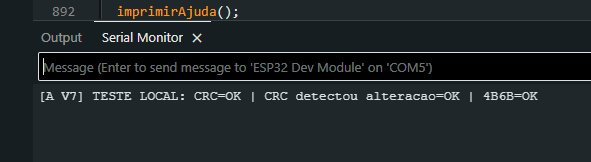
\includegraphics[width=\linewidth,height=150pt,keepaspectratio]{figuras/old_22_1.png}\caption{T01 — autoteste no circuito A.}\label{fig:old_22_1}\end{figure}
\begin{figure}[H]\centering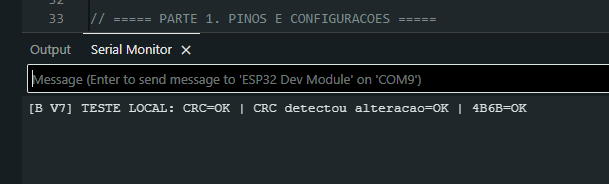
\includegraphics[width=\linewidth,height=135pt,keepaspectratio]{figuras/old_23_1.png}\caption{T01 — autoteste no circuito B.}\label{fig:old_23_1}\end{figure}
\begin{figure}[H]\centering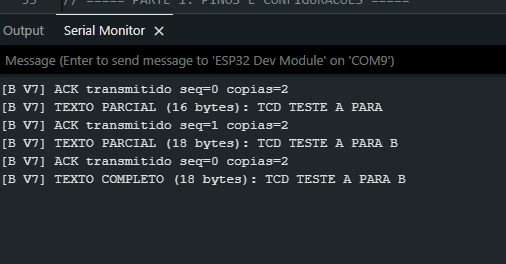
\includegraphics[width=\linewidth,height=180pt,keepaspectratio]{figuras/old_23_2.png}\caption{T02 — recepção da mensagem em B.}\label{fig:old_23_2}\end{figure}
\clearpage\subsection*{T03, T04 e T05}
\begin{figure}[H]\centering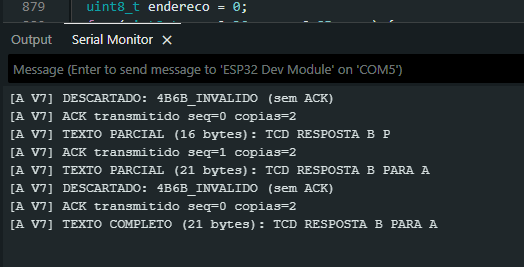
\includegraphics[width=\linewidth,height=190pt,keepaspectratio]{figuras/old_24_1.png}\caption{T03 — recepção da mensagem em A.}\label{fig:old_24_1}\end{figure}
\begin{figure}[H]\centering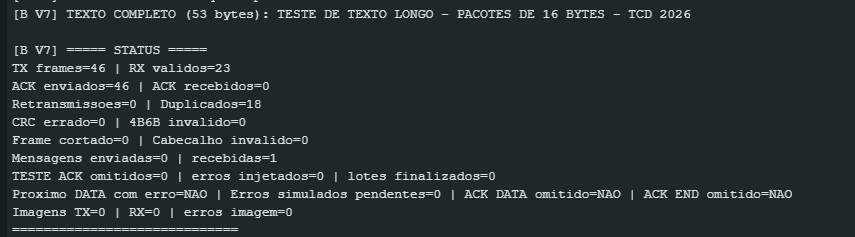
\includegraphics[width=\linewidth,height=145pt,keepaspectratio]{figuras/old_24_2.png}\caption{T04 — texto longo e contadores de B.}\label{fig:old_24_2}\end{figure}
\begin{figure}[H]\centering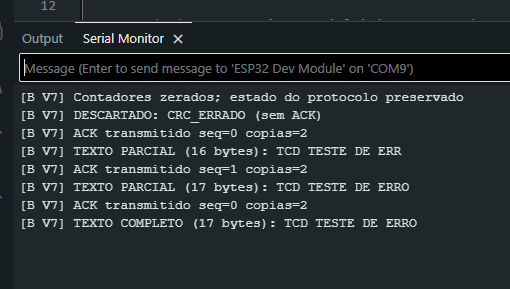
\includegraphics[width=\linewidth,height=195pt,keepaspectratio]{figuras/old_25_1.png}\caption{T05 — recepção do texto após erro simulado.}\label{fig:old_25_1}\end{figure}
\clearpage\subsection*{T06 e T07}
\begin{figure}[H]\centering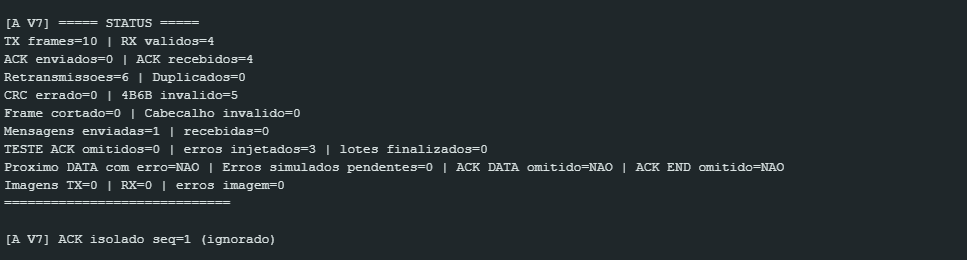
\includegraphics[width=\linewidth,height=130pt,keepaspectratio]{figuras/old_25_2.png}\caption{T06 — contadores do transmissor.}\label{fig:old_25_2}\end{figure}
\begin{figure}[H]\centering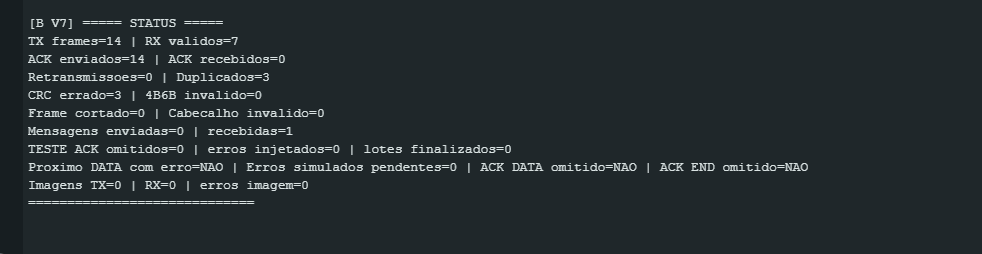
\includegraphics[width=\linewidth,height=130pt,keepaspectratio]{figuras/old_25_3.png}\caption{T06 — contadores do receptor, incluindo três erros CRC.}\label{fig:old_25_3}\end{figure}
\begin{figure}[H]\centering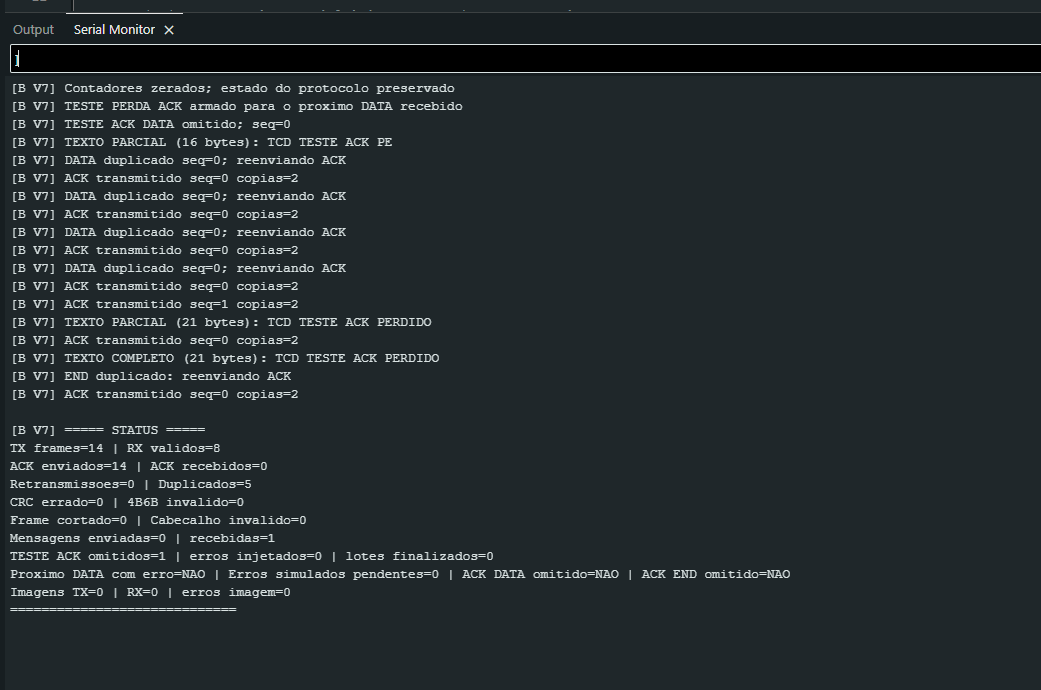
\includegraphics[width=\linewidth,height=230pt,keepaspectratio]{figuras/old_26_1.png}\caption{T07 — registro do transmissor.}\label{fig:old_26_1}\end{figure}
{\small T06: os três erros CRC estão registrados, mas o critério de duas mensagens não foi comprovado.\par}
\clearpage\subsection*{T07 e T08}
\begin{figure}[H]\centering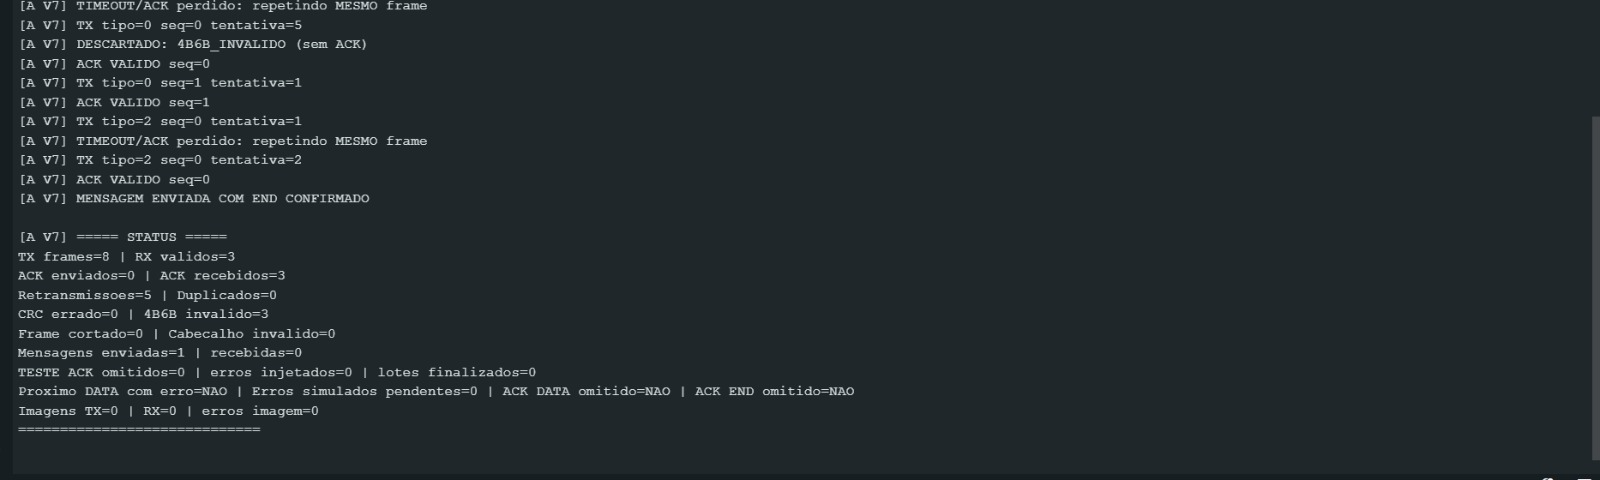
\includegraphics[width=\linewidth,height=185pt,keepaspectratio]{figuras/old_26_2.png}\caption{T07 — registro do receptor.}\label{fig:old_26_2}\end{figure}
\begin{figure}[H]\centering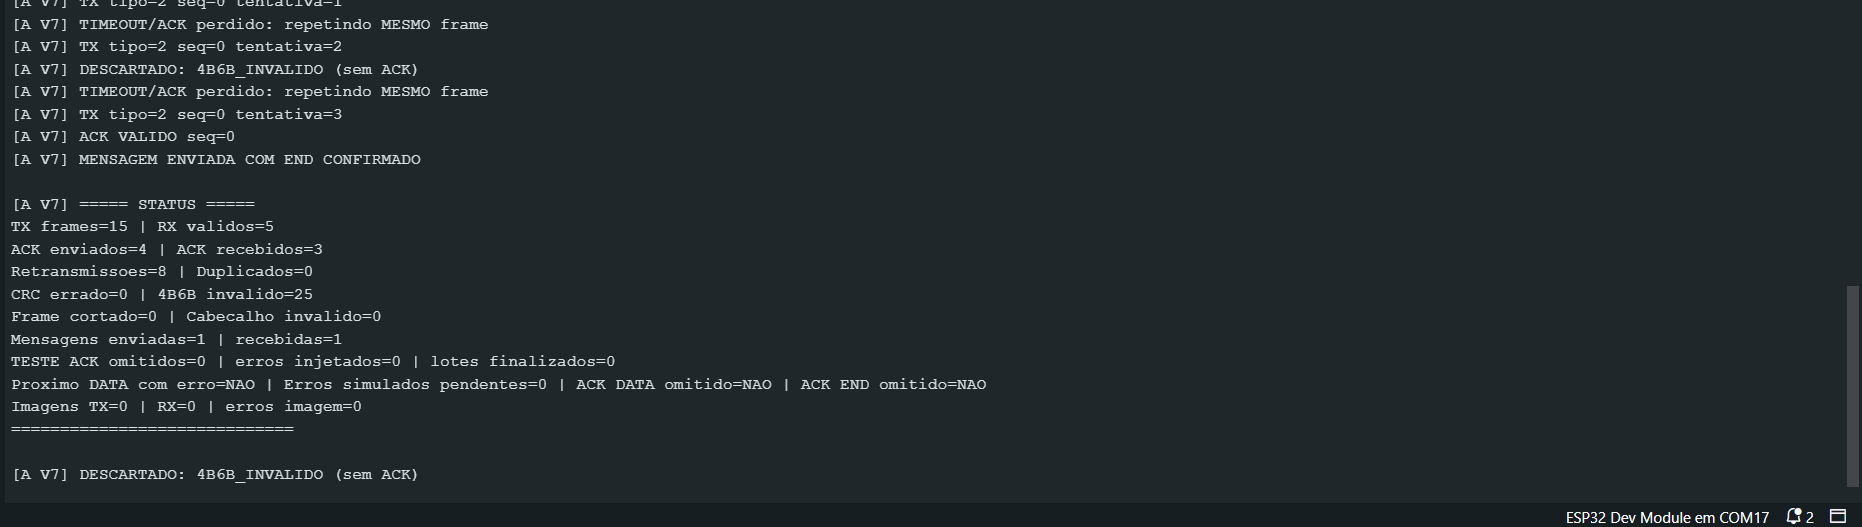
\includegraphics[width=\linewidth,height=185pt,keepaspectratio]{figuras/old_26_3.png}\caption{T08 — confirmação do END após retransmissão.}\label{fig:old_26_3}\end{figure}
\begin{figure}[H]\centering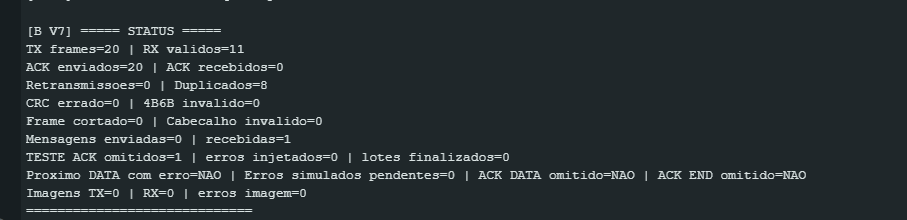
\includegraphics[width=\linewidth,height=180pt,keepaspectratio]{figuras/old_27_1.png}\caption{T08 — contadores do receptor e ACK omitido.}\label{fig:old_27_1}\end{figure}
\clearpage\subsection*{T09}
\begin{figure}[H]\centering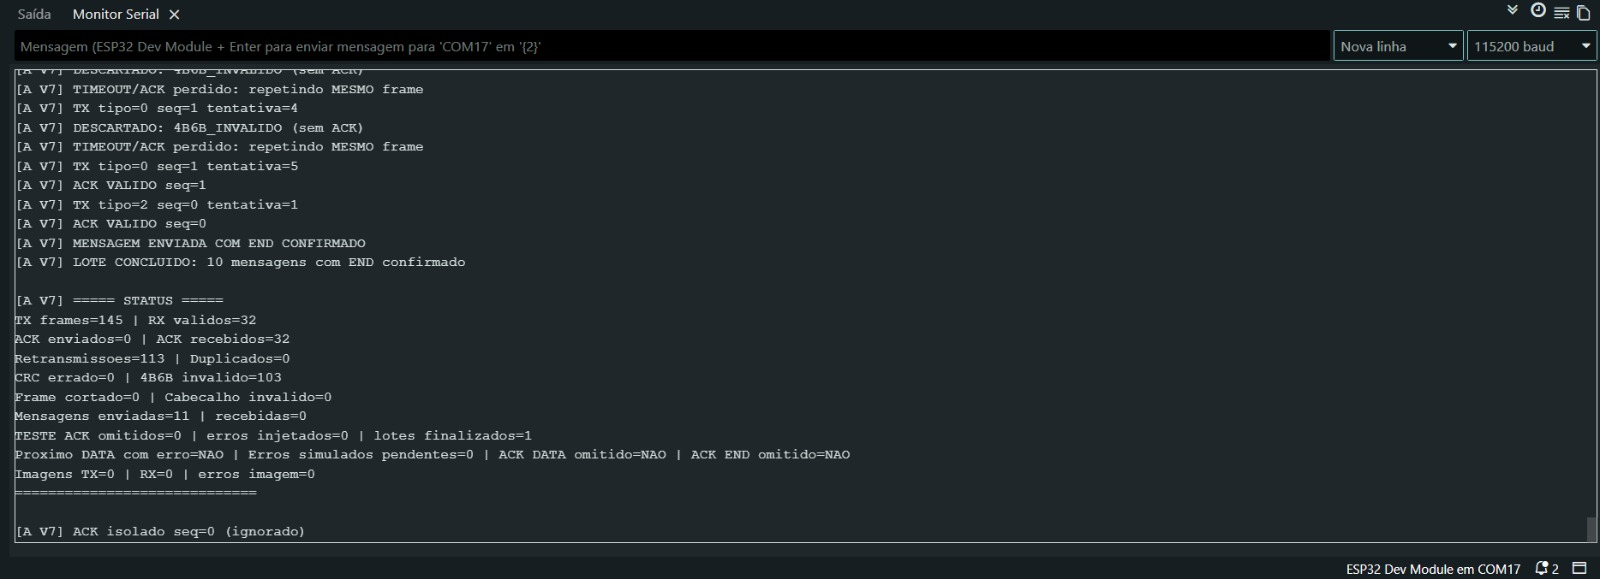
\includegraphics[width=\linewidth,height=180pt,keepaspectratio]{figuras/old_27_2.png}\caption{T09 — conclusão do lote no transmissor.}\label{fig:old_27_2}\end{figure}
\begin{figure}[H]\centering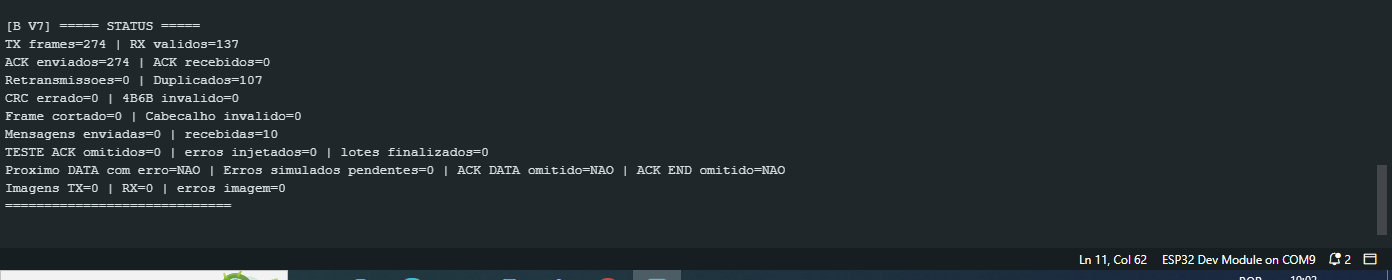
\includegraphics[width=\linewidth,height=180pt,keepaspectratio]{figuras/old_27_3.png}\caption{T09 — dez mensagens recebidas e duplicatas.}\label{fig:old_27_3}\end{figure}
\begin{figure}[H]\centering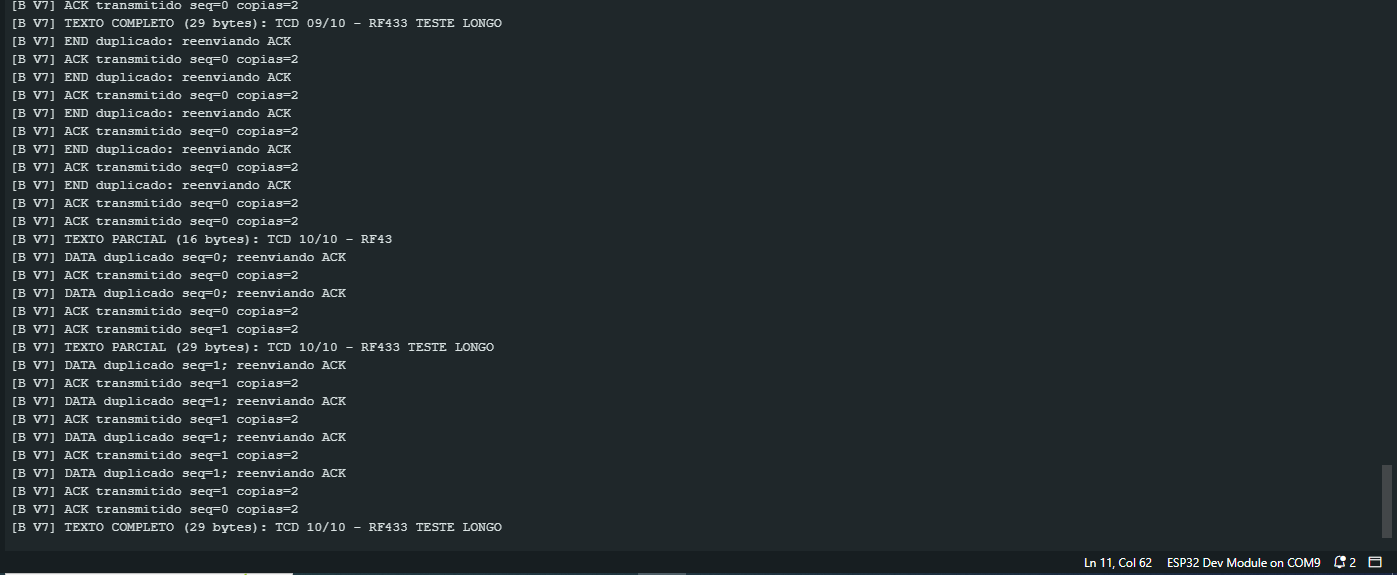
\includegraphics[width=\linewidth,height=180pt,keepaspectratio]{figuras/old_28_1.png}\caption{T09 — recepção das últimas mensagens do lote.}\label{fig:old_28_1}\end{figure}
{\small Os contadores do lote incluem atividade residual; os 113 reenvios não representam uma taxa isolada do T09.\par}

\clearpage\section{Relatório consolidado dos ensaios}
O relatório de ensaios de 24/11/2026, com 17 páginas, fornecido pela equipe, acompanha esta versão como documento complementar separado. Para evitar repetição, as evidências individuais permanecem no Anexo A e o PDF original é preservado sem alterações em \texttt{anexos/Relatorio\_Ensaios\_V7.pdf}. O documento inclui o protocolo de referência, procedimentos, resultados, registros T10–T14, fotos da trena e da mochila, capturas seriais, imagens reconstruídas, hashes, ficha consolidada e conclusão. Sua numeração interna e conteúdo foram preservados para rastreabilidade. \href{https://github.com/enzogomes2006/tcd-rf433-esp32/blob/main/relatorio/Relatorio_Ensaios_V7.pdf}{Consultar o relatório original de ensaios no GitHub}.

\subsubsection*{Índice interno do anexo}
\begin{table}[H]\centering\small\caption{Índice do relatório complementar de ensaios}\label{tab:21}
\rowcolors{2}{tcdlight}{white}\begin{tabularx}{\linewidth}{>{\hsize=0.6392\hsize\linewidth=\hsize\raggedright\arraybackslash}X>{\hsize=1.3608\hsize\linewidth=\hsize\raggedright\arraybackslash}X}
\rowcolor{tcdtablehead} \textcolor{black}{\textbf{Páginas do documento de ensaios}} & \textcolor{black}{\textbf{Conteúdo}} \\
1–2 & Objetivos, preparação da bancada e quadro-síntese. \\
3–5 & Procedimentos e resultados T01–T09. \\
6–7 & T10 — distância superior a 1 m, fotografias e logs. \\
8–9 & T11 — obstáculo passivo, comparação e logs. \\
10–11 & T12 — imagem 64\ensuremath{\times}32 A \ensuremath{\to} B e integridade. \\
12–13 & T13 — imagem 128\ensuremath{\times}64 A \ensuremath{\to} B e integridade. \\
14–15 & T14 — imagem 64\ensuremath{\times}32 B \ensuremath{\to} A, diagnóstico e integridade. \\
16–17 & Ficha consolidada, limitações, conclusão e imagem de referência. \\
\bottomrule\end{tabularx}\end{table}
O anexo deve ser interpretado juntamente com o corpo deste relatório, especialmente as ressalvas sobre T06, os tempos estimados, as condições variáveis e as capturas anteriores.


\end{document}
